\documentclass{article}
\usepackage[utf8]{inputenc}
\usepackage{todonotes}
\usepackage[colorlinks=true, allcolors=blue]{hyperref}
\usepackage{algorithm}
\usepackage{algorithmic}
\usepackage{multirow}


\title{rapport}
\author{jjycavailles }
\date{May 2019}

%\usepackage{natbib}

%\usepackage[authoryear]{natbib}
%\usepackage{biblatex}
\usepackage[round]{natbib}
%\usepackage{natbib}

%\bibliographystyle{plainnat}
%\usepackage[round]{natbib}

%\usepackage{cite}
%\setcitestyle{authoryear, open={((},close={))}

%\bibliography{references.bib}
%\bibliography{intro.bib}
%\addbibresource{intro.bib}
%\bibliographystyle{apalike}
%\usepackage[style=authoryear]{biblatex}
%\setcitestyle{authoryear,open={((},close={))}}

%\bibliographystyle{apalike}


\usepackage{graphicx}


%\usepackage{hyperref}
\usepackage[colorlinks=true, allcolors=blue]{hyperref}





\begin{document}

\begin{titlepage}

\begin{center}
  
\includegraphics[width = 25mm]{LogoInsa.png} \hfill
  
\includegraphics[width = 30mm]{logo_cnrs.jpg}
\end{center}

%\title{\textbf{Rapport de stage} \\ Ingenieur en mathematique \\ \textbf{ etude de la classification en regimes de temps et de leurs impacts pour des utilisations metiers.} }
%\author{Jerome Cavailles \\ $4^{ieme}$ annee, Genie mathematique et modelisation \\ INSA Toulouse}
%\date{28/06/2018 - 07/09/2018}




\vspace*{1cm}

\begin{center}
\rule{\linewidth}{0.7mm} \\
[0.4cm]
\textbf{ \Huge Internship report} \\
[0.2cm]
\large \emph{Engineer in mathematics} \\ 
[0.6cm]
\textbf{ \huge Destabilizing effects of controlling ecosystem behavior} \\
[0.4cm]
03/01/2019 - 08/30/2019 \\
[0.4cm]
\rule{\linewidth}{0.7mm}
\end{center}

\vspace*{0.5cm}

\begin{center}
\textbf{\Large{Jerome Cavailles}} \footnote{\url{jcavaill@etud.insa-toulouse.fr}} \\ [0.3cm] $5$ years, Mathematical engineering and modeling %\\ INSA Toulouse
\end{center}

%^{\text{ieme}}

%\maketitle

%\vspace*{2.5cm}
\vspace*{1.9cm}

\begin{flushleft}
Supervisor : Yuval Zelnik \footnote{\url{yuval.zelnik@sete.cnrs.fr}} \hfill
Tutor : Marie-Hélène Vignal \footnote{\url{marie-helene.vignal@math.univ-toulouse.fr}} \\  
Michel Loreau \footnote{\url{michel.loreau@sete.cnrs.fr}} \hfill
Charles Dossal \footnote{\url{dossal@insa-toulouse.fr}} \\
Laboratory : CNRS-Moulis \footnote{2, route du CNRS - 09200 Moulis, France, \url{http://www.cbtm-moulis.com}} \hfill 
University : INSA Toulouse \footnote{135, Avenue de Rangueil 31077 Toulouse Cedex 4, \url{http://www.insa-toulouse.fr}} \\
\hfill Paul Sabatier \footnote{118 route de Narbonne, 31062 Toulouse Cedex 9, \url{http://www.univ-tlse3.fr/}}
\end{flushleft}

%\paragraph{}
%\begin{tabbing}
%\hspace{2cm}\=\hspace{6cm}\=\hspace{2cm}\=\kill
%Supervisor \> Yuval Zelnik \footnote{\url{yuval.zelnik@sete.cnrs.fr}} \>
%Tutor \> Marie-Hélène Vignal \footnote{\url{marie-helene.vignal@math.univ-toulouse.fr}} \\  
%\> Michel Loreau \footnote{\url{michel.loreau@sete.cnrs.fr}} 
%\> \> Charles Dossal \footnote{\url{dossal@insa-toulouse.fr}} \\
%Laboratory \> CNRS-Moulis \footnote{2, route du CNRS - 09200 Moulis, France, \url{http://www.cbtm-moulis.com}} \> University \> INSA Toulouse\footnote{135, Avenue de Rangueil 31077 Toulouse Cedex 4} \\
%\>\>\> Paul Sabatier \footnote{118 route de Narbonne, 31062 TOULOUSE CEDEX 9 \url{http://www.univ-tlse3.fr/}}
%\end{tabbing}

\end{titlepage}



\newpage
\addcontentsline{toc}{section}{Abstract}
\section*{Abstract}
\paragraph{}
\todo{}

\paragraph{Keywords}



\newpage
%\addto\captionsfrench{\def\contentsname{}} % pour supprimer le "table des matieres en haut"
\paragraph{}
%\section*{Contents}
\addcontentsline{toc}{section}{Contents}
\tableofcontents



\newpage
%\section*{Liste des figures, des tables et des algorithmes}
%\addcontentsline{toc}{section}{Liste des figures, des tables et des algorithmes}
%\paragraph{}
\addcontentsline{toc}{section}{List of figures}
\listoffigures


\listoftables

\listofalgorithms

\newpage
\addcontentsline{toc}{section}{Abbreviations /Glossary}
\todo{use nomenclature packages}
\section*{Abbreviations / Glossary}
%\listoffigures


\newpage
\addcontentsline{toc}{section}{Preface}
\section*{Preface}
\todo{why this report, why this internships, why this subjects, ...}


\newpage
\section*{Acknowledgment}
\addcontentsline{toc}{section}{Acknowledgment}



\newpage
%\todo{Choice of this internship ?}
\section*{Introduction}
\addcontentsline{toc}{section}{Introduction}

\subsection*{Station presentation}
\addcontentsline{toc}{subsection}{Station presentation (1-2 pages)}

\paragraph{}
The CNRS\footnote{\url{http://www.cnrs.fr/en/cnrs}}, the Scientific Research National Center (in french, Centre National de la Recherche Scientifique) was created on the 19th of October, 1939. It is a world renowned research institution, ranked second by  nature index \footnote{\url{https://www.natureindex.com/institution-outputs/generate/All/global/All/n_article}}. It has approximately 33,000 researchers working in 1,144 laboratories throughout France and abroad, with a budget around 3 billion euros. 

The CNRS is currently headed by Antoine Petit (President and CEO), and its laboratories are organised in two types: proper units (UPRs) and mixed units (UMRs), the latter being managed in association with other French institutions (higher education establishment or another research institution). In addition, there are 36 international Joint Units (UMI) of collaborations around the world. The CNRS conducts research in all disciplines of basic research (Ecology and environment, Humanities and social sciences, Engineering and systems, Mathematics, Physics, Information sciences, etc. , ).


\paragraph{}
One of these mixed research units (UMR 5321) is the Station for Theoretical and Experimental Ecology\footnote{\url{https://sete-moulis-cnrs.fr}} (SETE), located in Moulis\footnote{\url{http://www.communes.com/midi-pyrenees/ariege/moulis_09200/}} (Ariege, France). It was originally founded in 1948 by professors Jeannel and Vandel, due to its vicinity to many caves, with the aim of the station to use the underground cave systems in order to study the formation and physical properties of karstic systems as well as systematics and adaptations in hypogeaic organisms. More recently, under the direction of Jean Clobert\footnote{\url{http://www.sete.cnrs.fr/spip.php?article26}}, the station transitioned to perform more general research about ecology.

The research station is now directed by Michel Loreau\footnote{\url{http://www.cbtm-moulis.com/m-171-michel-loreau.html}}, and has a staff of 60 persons working in it, along several axes. 
Firstly, the evolutionary ecology group study empirically "how biodiversity is generated and how species adapt to new contexts" \footnote{\url{https://sete-moulis-cnrs.fr/en/research/evol}}. Another group called "Eco-Evolutionary Dynamics in changing Landscapes "aims at understanding reciprocal eco-evolutionary dynamics in landscapes modified by human activities" \footnote{\url{https://sete-moulis-cnrs.fr/en/research/eedyl}}.


%Firstly, the consequences of global changes to biodiversity integration is studied, notably by using empirical data \footnote{\url{http://www.ecoex-moulis.cnrs.fr/spip.php?article3}}. Another axis is the study on phenotypic plasticity (which permit a faster adaptation to environmental change than genetic adaptation) \footnote{\url{http://www.ecoex-moulis.cnrs.fr/spip.php?article4}}. Environmental variation is still consider to monitor the impact to social interactions \footnote{\url{http://www.ecoex-moulis.cnrs.fr/spip.php?article94}}. Also, the conservation and management of land and studied both experimentally and theoretically \footnote{\url{http://www.ecoex-moulis.cnrs.fr/spip.php?article79}}.
%biodiversity and ecosystem functioning, conservation and land management, social interactions, environmental variation and evolution, phenotypic plasticity. 
%% = YZ: It would be good to define the axes more properly and concisely
%% the team are changing, 

Several unique experimental platforms are located in the station. A laboratory inside the cave system is still operational, a $750m^2$ greenhouses have been constructed, a $520m^2$ aviary with an automatic system for data capture using video and sensors.
The station also has equipment for molecular biology, cell biology, physiology, for surgery and also to breeding of invertebrates, fish, amphibians, and reptiles. However, the most unique facility is the metatron\footnote{\url{https://themetatron.weebly.com/}}, which is a network of 48 cell.  
%% = YZ: This phrasing "network cell semi-controlled" is strange. You might want to mention size and such things, to give the reader an idea of what it is. You can even add a photo here, perhaps.
With a surface of $100m^2$ and a height of 2 m, each unit reproduce a small ecosystem, with different vegetation (50 species per cage) and invertebrate (40 families per cage). Cells can be linked to study the dispersal of the species from one cell to others. By controlling the temperature, it is possible to investigate the consequences of the global change. For example, a gradient of temperature can be applied to monitor the distribution of different populations.


Another unique facility is the aquatron. Same as the metatron, it is a network of interconnected cell. Each cell (144) are a basin of less than $2m^3$ used to study the impact of climate change on aquatic species.




\begin{figure}[h]
\begin{center}
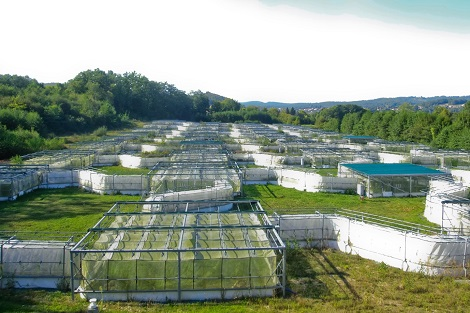
\includegraphics[width=6.cm]{metatron_0.jpg}
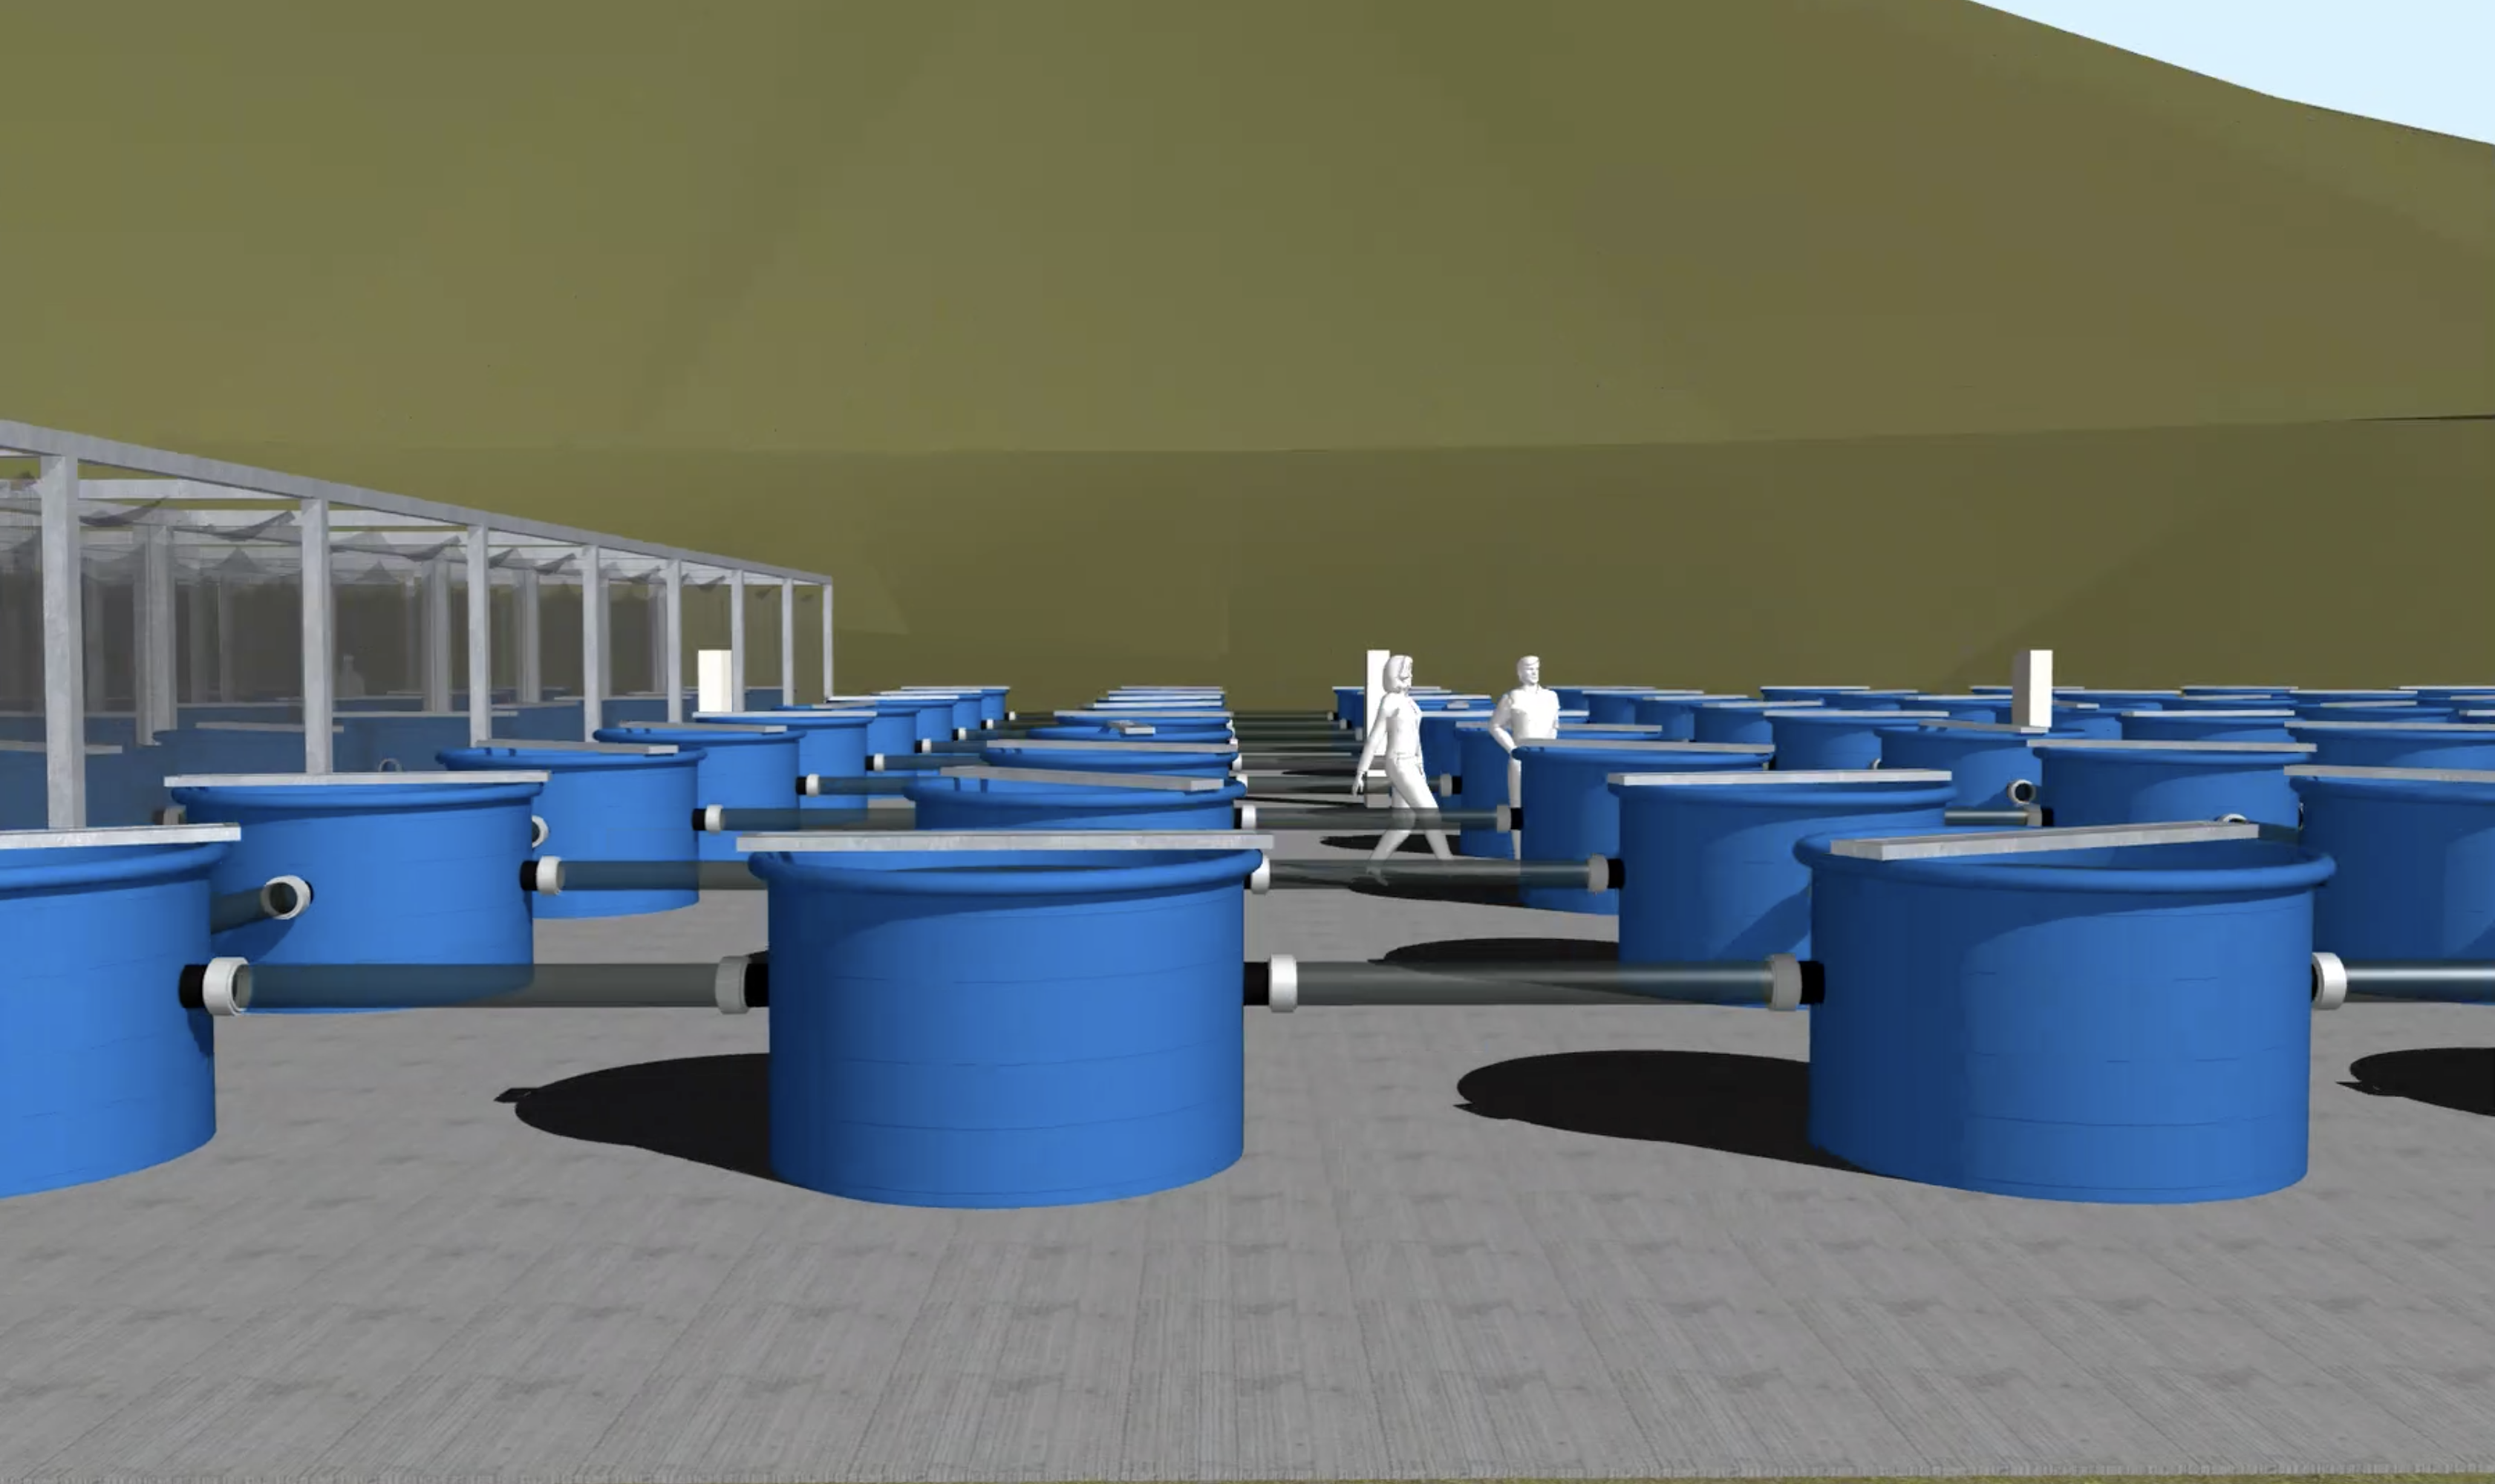
\includegraphics[width=6.cm]{aquatron.png}
\end{center}
\caption{\label{fig:temp}Left : Metatron, right : Aquatron}
\end{figure}

%% YZ: There's also the aqua-tron, that has recently been finished. You can talk to several people in Jose's team about it, if you're interested.


\paragraph{}
%Since 2012, the station hosts the Centre for Biodiversity Theory and Modelling (CBTM) \todo{now renamed Linking ...}
The centre for biodiversity theory and modelling (CBTM) \footnote{\url{http://www.cbtm-moulis.com}} 
%% YZ: Actually, not quite. The CBTM should still exist as a separate entity, in parallel to the "linking team". I think for your concerns, it might be simpler to just describe the CBTM...
aims to unify theories of biodiversity changes and of their consequences, in order to address the major challenges of the present biodiversity crisis.
%% YZ: I think you can say more than the previous sentence...
Lead by Jose M. Montoya\footnote{\url{http://www.cbtm-moulis.com/m-224-jose-m--montoya.html}}, the research ranges from phylogenetics to human interactions. Indeed, the ambition of the team is to give a theoretical framework to a general biodiversity science in order to deal with the present biodiversity crisis\footnote{\url{https://www.ipbes.net/news/Media-Release-Global-Assessment-Fr}}.

In practice, the team focus on several axes : generation of biodiversity and ecosystem services, the human nature interactions, habitat fragmentation and stability of ecological systems.

%% YZ: I guess you should state the axes right here. Otherwise, it is quite hard to follow.
The first axis focus on trying to understand how biodiversity change will affect ecosystem services. For example, how the loss of a species can affect crop production. However, because ecology and evolution theory are interrelated, the team integrates the role of eco-evolutionary dynamics in the responses of environmental changes. The same work is done for structure, dynamics and function of ecosystem, which are also interconnected \citep{bastazini_loss_2017} \cite{bideault_temperature_2019} \cite{galiana_geographical_2019}.



An additional axis is of human-nature interactions, which is studied in both directions : the human impact on biodiversity (habitat loss, fragmentation, global warming, etc.) which represent a threat of at least one in six species during this century, but also the feedback of biodiversity loss on human society. The aim is to study the long term sustainability of coupled social-ecological systems. Another objective is to better understand how biodiversity changes affect the services of the ecosystem, in particular  crop production and biological control in agricultural landscapes \cite{cazalis_we_2018} \cite{lafuite_sustainable_2018} \cite{montoya_trade-offs_2018} \cite{montoya_tradeoffs_2019}

% Habitat fragmentation and spatial dynamics of biodiversity
A particular case of human impact, landscape fragmentation which occurs at multiple spatial scales, is itself a subject of research: the habits loss itself as well as its effect ton he spatial dynamics of the ecosystem, with a special attention to metacommunities dynamics \cite{goncalves_habitat_2018} \cite{jacobi_operationalizing_2018}.

% Biodiversity and stability of ecological systems
Finally, a major focus of the team is studying the stability of ecological systems\footnote{\url{http://www.cbtm-moulis.com/m-214-biostases.html}}. Stability is an important feature of the ecosystem, and is a notion that is used in all previous research axes mentioned. The main research focus is to understand and quantify stability both in time and in space \cite{wang_stability_2017} \cite{zelnik_impact_2018}. However, since different stability measures are used in theory and experimental ecology, the team has tried to bridge the gap between these different measures and thus unify the notion of the stability \cite{arnold_examination_nodate}.
%% YZ: I am not sure barbier2019pyramids makes sense here. What measures is it bridging?
Different aspect of stability are studied: the link between the diversity of a species community and the stability of the community \cite{vallina2017phytoplankton}, the stability of meta-ecosystems \cite{arnoldi_particularity_2016} \cite{lurgi_effects_2016} \cite{wang_biodiversity_2016}.
Again, the sustainability of coupled social ecological systems are studied, in particular the role of human behavior in preventing the possible collapse of this systems.
%in as stability point of view (averting collapse for example).
%% YZ: This last sentence is quite strange.
Moreover, a mathematical framework is built by exploring the different notions of stability in order to link them \cite{arnoldi2016unifying} \cite{donohue_navigating_2016} and to know how to predict a critical changes by using experimental measures such as temporal variability \cite{arnoldi2016resilience} \cite{haegeman_resilience_2016} \cite{wang_invariability-area_2017}. 
% citation jusqu'a 2016 inclus



\newpage


\subsection*{Context}
\addcontentsline{toc}{subsection}{Context}







\subsection*{Ecosystem stability} % monitoring ?
\addcontentsline{toc}{subsection}{Ecosystem stability}

\paragraph{}
Ecosystems around the world are facing unprecedented disturbances due to increasing human intervention \cite{oosthoek_humanity_2005}. It is therefore important to analyse  their dynamics in the context of human perturbations, in order to both predicts the following state of the ecosystem and also to better manage it.
% complex dynamics
Nevertheless ecosystem dynamics can be notoriously complex, in particular due to the interactions between the different interconnected elements that constitute the system. %Thus, it is unavoidable to consider integrative study. 

\paragraph{}
\label{stability_litterature}
Ecologists are often interested in estimating stability far from equilibrium (as opposed to the classical physics approach, which focuses on studying stability near the equilibrium). Therefore, ecology needs to develop news tools to deal with understanding and predicting stability in complex dynamical systems. 
% resilience
One such concept, resilience, is traditionally used in theoretical studies, but is not the most relevant %\cite{arnoldi2016resilience}
\cite{gunderson_ecological_2000} \cite{neubert_alternatives_1997}.

Other stability measures are used to quantify the health of an ecosystem and follow its development over time, and are used to set accurate goals for the future planning management \cite {donohue_navigating_2016} \cite{mayer_strengths_2008}. A difficulty is that this word is used for many different meanings. One study has identified 163 definitions of 70 different stability concepts \cite{grimm_babel_1997}.

However, according to the same study, all these can be collapsed to only 6 pertinent concepts (constancy,  resilience,  persistence,  resistance,  elasticity and domain of attraction). Nonetheless, even if it is possible to reduce the number of the stability notions, several of them need to be used in order to consider the various aspects of stability, so as not to lose information on the behavior of the ecosystem \cite{derissen_relationship_2011}. There is thus a compromise between using too few measures, which will not capture all the relevant information, and using too many measures, which will not be practicable and may still not catch all the information \cite{hillebrand_decomposing_2018} \cite{donohue_dimensionality_2013}.
%Indeed, different stability measures have been defined to monitor different aspects of the system's response to perturbations. 
%If this different measures appear to be strongly related, it is not always true \cite{donohue2013dimensionality}.





%\paragraph{ecosystem management \\}
\paragraph{}

These different concept a main interest for ecosystem management \cite{mumby_ecological_2014}. It serves to anticipate the consequences of disturbances, in particular for anthropocentric ones. In the past decades, the field of ecosystem management has grown rapidly \cite{grumbine_reflections_1997} in response to the various modern disturbances, in order to sustain the integrity of ecosystem (including its structure, composition and function) \cite{jensen1994overview}. 

A major obstacle is to define measurable goal in order to have clear and trackable progress \cite{slocombe_forum:_1998}.
Even if it remains impossible to know all the exact processes operating within the ecosystem, it is still possible to understand the dominant behavior, which could be sufficient for ecosystem management \cite{mori_ecosystem_2011} \cite{slocombe_forum:_1998} \cite{stanley_ecosystem_1995}.
%\cite{mori2011ecosystem, slocombe1998defining, stanley1995ecosystem}







\subsection*{Forest fire}
\addcontentsline{toc}{subsection}{Forest fire}

\paragraph{}
As detailed previously, ecosystem  dynamics  can  be  notoriously  complex, in order to study the link between different notions of stability, a case studied is choose. 
We focus on forest fire management, as the dynamics of both forest and fire are well established. Nonetheless, the repercussions of fire management in forests, are not well understood, with much to be explored.


\paragraph{}
%\paragraph{forest disturbance \\}

Forest dynamics are affected by various disturbances. We define disturbance as events that can cause significant changes to the ecosystem \cite{white1985natural} \cite{rykiel_towards_1985} . Disturbance play an important role in forest ecosystem, notably by generating heterogeneity in the landscape \cite{turner2010disturbance}.

Disturbances can be defined by their duration \cite{perera_simulation_2015}. First, the disturbance who are considered instantaneous comparative to the dynamics of the forest (e.g. flood, windstorm, pest outbreaks ...).
Second, the constrain on long term, such as drought, temperature fluctuation or grazing.

Another useful distinction is the implication of human in the disturbance, even if it is not possible to isolate anthropogenic perturbations from natural ones \cite{perera_simulation_2015}.
Indeed, the human impact increases with time. For example, the area logged per year in Canadian forests has doubled between 1960 and 1995 \cite{smith_canadas_2000}. This logging disturbance could be relatively different from the natural ones.

%Also, some particular perturbations can be differentiate, the severe but rare events, this are termed "LIDS" for large and infrequent disturbances \cite{foster1998landscape}.
% rephrase if used this sentence. 

Finally, this different perturbations are often interrelated \cite{keane2015exploring}. This could create synergism between them \cite{mandre_environmental_2011} or have unanticipated responses \cite{perera_simulation_2015}. For example, fire and climatic fluctuations could interact to product cumulative effects \cite{romme_historical_2009}.



%\paragraph{Forest management \\}
\paragraph{}
For decades, sustainable forest management (SFM) has been used to maintain forest ecosystems \cite{macdicken_global_2015}. 
This practice serves to maintain different aspect of the ecosystem such as productive functions, biological diversity, and socioeconomic functions \cite{makela_using_2012}. 
However, its main target is to conserve the forest ecosystem as an unified entity. %\cite{franklin1989toward}.
%Moreover, there is no unanimity on this different facet of sustainability \cite{martinez-vega_assessing_2016}.
Also, the human demands from forests have broadened, making forest management more complex \cite{eggers_balancing_2017}. Several recent studies have shown that ecosystem management should try to reproduce the nature disturbance in order to preserve the dynamics of the forest \cite{bengston_changing_1994} \cite{bengtsson_biodiversity_2000}. 
According to \cite{hunter1990wildlife} and \cite{hunter1988paleoecology} it could be possible to imitate the size, frequency and severity of disturbances.

To reach this different target (mainly sustainability and productive functions), various criteria are used. To be practical, such criteria need follow some rules: be easily measured, be sensitive to stress, be anticipatory (to counter change), be integrative (consider different facets of forest ecosystem such soils, vegetation types ...) and have a low variability in response \cite{dale_challenges_2001}. However, monitoring programs typically consider only few indicators and fail to take into account the complexity of the ecosystem \cite{dale_challenges_2001}.


%\paragraph{Fire \\}
\paragraph{}

One on the main disturbances in forests is fire, and in some regions, it is the most significant one. Fires can create spatial patterns and heterogeneity in the landscape \cite{skinner_overview_nodate}. Fires also affect plant behavior, such that plants develop traits for adaptation to fire (thick  bark  and fire-stimulated flowering, sprouting, seed release and/or germination) \cite{mckelvey1996overview} \cite{chang1996ecosystem}.

Fires are also linked with other perturbations, mostly climatic variation \cite{mckenzie_climatic_2004}\cite{da2018dynamics}, by its effects to on fuel \cite{schoennagel_interaction_2004} and by weather \cite{fernandes_fire-smart_2013}. In practice, in some regions, fires are greatly affected by humans, wildfires have been considerably reduced due to the intervention of firefighters. Different management practices are used, depending notably on the country and the tree species, and mostly based on the misconception that lock the dynamics of a system will prevent it from collapse. That is why variability and collapse probability are the two measures choose in this study. In order to restore the natural dynamics of the forest, fires are sometimes allowed to run their course freely without intervention \cite{wallenius2011major}. 

Finally, one of the problem of the study of fire is its stochastic aspect and the variability in both space and time, which add complexity to the modelling of fire events and dynamics \cite{agee1998landscape} \cite{lertzman1998three}.

\newpage

\todo{expend (later)}

\subsection*{Synopsis}
\addcontentsline{toc}{subsection}{Synopsis}

\paragraph{}
The main purpose of the present document is to exhibit an ecosystem case where different notions of stability do not behave similarly. In order to do this, we look at how variability and collapse probability change with various model parameters, we consider different dynamical cases of the system, and describe the consequences for management practices.











%%%%%%%%%%%%%%%%%%%%%%%%%%%%%%%%%%%%%%%%%%%%%%%%%%%%%%%%%%%%%%%%%%%%%%%%%%%%%%%%%%%%%%%%%%%%%%%%%%%%%%%%
% Methods
%%%%%%%%%%%%%%%%%%%%%%%%%%%%%%%%%%%%%%%%%%%%%%%%%%%%%%%%%%%%%%%%%%%%%%%%%%%%%%%%%%%%%%%%%%%%%%%%%%%%%%%%

\newpage
\section{Methods}


\subsection{Model}


\paragraph{}
We consider a model of a forest fire, with $N$ being live biomass and $W$ dead wood. The living biomass is defined like standing alive tree and dead wood is dead wood debris and standing dead trees \cite{russell2015quantifying}.

The living biomass follow a logistic growth \cite{tsoularis2002analysis} \cite{jensen1975comparison} with an allee effect \cite{stephens1999allee} \cite{amarasekare1998allee}. On the other hand, the evolution of the dead wood is proportional to the density of $N$ and decay with time \cite{kahl_wood_2017} \cite{shorohova_stump_2012} \cite{christensen_estimation_1977} \cite{delaney_quantity_1998} \cite{barbosa_decomposition_2017} \cite{fravolini_quantifying_2018} \cite{wilson_dynamics_2005} \cite{zielonka_dynamics_nodate}.

Both $N$ and $W$ are affected by fire, with a stronger effect for $W$ (the dead wood burn easier than $N$). A fire occur when $t\in F$ the set of fire events. The severity of the fire is assumed to follow an exponential law of average $strength$. Finally, the severity of the fire is proportional the density biomass $N$ and $W$ with a greater importance for $W$ \cite{martinson_fuel_2013} \cite{safford_effects_2009} \cite{lecomte_effects_2006}.

\paragraph{}

\[
\left\lbrace
\begin{array}{rcl}
\frac{dN}{dt} & = & gN(1-N/K)(N/a-1) - \delta_F(t)s(t)(N+\alpha W) \\
\\
\frac{dW}{dt} & = & mN -dW - \beta\delta_F(t)s(t)(N+\alpha W) \\
\end{array}
\right.
\]

The major assumption of the model is that fire frequency is independent of fuel density, it will be argued later that do not question the following results of this study.

Another assumption is that fire need fuel ($W$) to burn. In other words, when $W=0$, fire stop. It is based on the fact that fire are manly driven by fuel \cite{schoennagel_interaction_2004} \cite{stephens_effects_2012} \cite{syphard_comparing_2011} \cite{safford_effects_2009} \cite{stephens_experimental_2005}.

Also, we consider only density biomass and do evaluate the spatial distribution of both density and fire severity \cite{bergeron_natural_2002}.

Same, we consider only one type of forest. Indeed, it have been argued that different type of forest fire could be differentiate (crown fires, light surface fires ... ) \cite{heinselman1981fire}.
% fire severity proportional to the density of $N$ and $\alpha W$ 


\paragraph{}
\todo{useful to give value ? (and justify with paper) it is not that simple, it could be a mess ...}
\todo{all value at least positive non null, and m lower than max(dn / dt)}

This model used $9$ parameters, 5 for growth therms and 4 for the fire model.

The first one $g$ is the grow rate of the living biomass. $K$ is the forest's carrying capacity. 

The allee effect threshold $A$ represent the minimum quantity of living biomass in order to survive. In other words, if the dynamics of $N$ go below $A$, the system collapse. The possible value of $A$ are between $0$ and $1$, but in practice $A$ take low value, typically between $0.02$ and $0.2$.

For the growth part of dead wood, $m$ is the decay rate of living biomass (the rate of conversion from $N$ to $W$) and $d$ the decay rate of $W$ itself.

Now, for the fire term, $\beta$ is the coefficient that represent the fact that $W$ burn easier than $N$. $\delta_F(t)$ and $s(t)$ represent respectively the fire occurrence and the severity of an eventual fire at the time $t$. \todo{beta and alpha bigger than $1$}

Finally, similar to $\beta$, $\alpha$ represent the fact that $W$ burn easier than $N$.





\paragraph{}
In order to simplify the study of the model, we adimensionnalise the system. We have anymore only 7 parameter (\hyperref[adim]{calculus in appendix}). The adimensionnalise system is the following :

\[ % adim model
\left\lbrace
\begin{array}{rcl}
\frac{dN}{dt} & = & N(1-N)(N-A) - \delta_F(t)s(t)(N+\alpha W) \\
\\
\frac{dW}{dt} & = & mN -dW - \beta\delta_F(t)s(t)(N+\alpha W) \\
\end{array}
\right.
\]

\paragraph{estimation of "reasonable" coefficient for this model%, sometimes easier to find "reasonable" coefficient, $K$ not anymore present, but not always ...
} \todo{}


%\paragraph{Remark} % equilibrium
\paragraph{} % equilibrium
To help understand the dynamics of the model used, we give some simple analytic result. to do this, we only consider growth terms.

\[ % adim model
\left\lbrace
\begin{array}{rcl}
\frac{dN}{dt} & = & N(1-N)(N-A) \\
\\
\frac{dW}{dt} & = & mN -dW \\
\end{array}
\right.
\]

\todo[color = purple]{reflechir à ce que je met en annexes} 

\paragraph{}
We have thus 3 equilibrium, 2 stable $(0, 0)$ and $(1, \frac{m}{d})$ and one unstable $(A, \frac{mA}{d})$ (\hyperref[equi]{calculus in appendix}).

\paragraph{}
Also, the figure below give an example for a well choose set of parameters of a time series. We can see that here the dynamics come back to the stable equilibrium $(1, \frac{m}{d})$ most of the time, except for the last fire when the system collapse to go to the other stable equilibrium $(0, 0)$. \todo{strength the temporal series (final time = 300)}

\begin{figure}[h!]
\centering
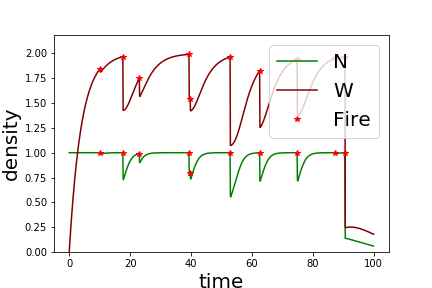
\includegraphics[width=6cm]{return_between_2.png}
\caption{Time series example}
%\label{fig:universe}
\end{figure}

\newpage
\paragraph{}
Also we represent the phase portrait for both $N$ and $W$. We recall that the dynamics of $W$ depend of the value $N$. 
%%%%% same parameters set for both

\begin{figure}[h!]
\centering
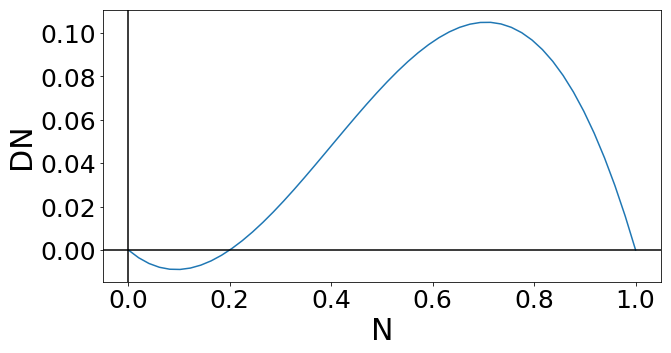
\includegraphics[width=6cm]{phase_N.png}
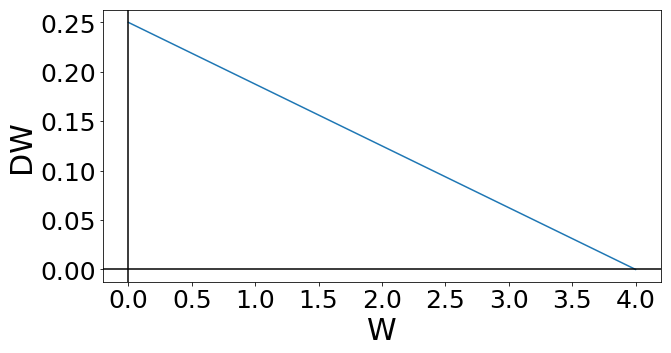
\includegraphics[width=6cm]{phase_W.png}
\caption{Phase portrait}
%\label{fig:universe}
\end{figure}

\paragraph{}
We can remark that the growth of the system is continuous and deterministic. However, the perturbation (fire) are discrete and stochastic. The implementation to solve the sytem need thus to take care of this, more details in \hyperref[technicality]{appendix}.
%\todo{I have already 2-3 papers about this, re found, cite}




\paragraph{}
\label{average_estimation}
Also, in order to not have to run too long simulation, an average of both $N$ and $W$ is estimated. It help to initialise the dynamics, indeed the transitions time is shorter

An analytic expression is given, mainly based on the assumptions that frequency is high enough to consider that the global dynamics of the system is continuous (\hyperref[average]{calculus in appendix}).


\[
\left\lbrace
\begin{array}{rcl}
N^{av} & = & \frac{1+a+\sqrt{(1-a)^2-4\gamma}}{2} \\
W^* & = & \epsilon N^* \\
\end{array}
\right.
\]

With,
\[
\left\lbrace
\begin{array}{rcl}
\epsilon & = & \frac{m-\beta s f}{d + \beta s f \alpha} \\
\gamma & = & sf(1+\alpha\epsilon)
\end{array}
\right.
\]

\paragraph{}
We can check below that average are well estimated, even for low value of frequency.

\begin{figure}[h!]
\centering
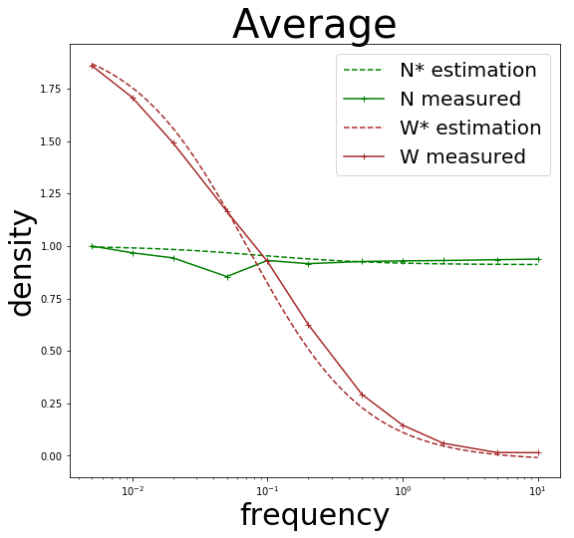
\includegraphics[width=9cm]{average.png}
\caption{Average $N^{av}$ and $W^{av}$}
%\label{fig:universe}
\end{figure}




%%%%%%%%%%%%%%%%%%%%%%%%%%%%%%%%%%%%%%%%%%%%%%%%%%%%%%%%%%%%%%%%%%%%%%%%%%%%%%%%%%%%%%%%%%
%%%%%%%%%%%%%%%%%%%%%%%%%%%%%%%%%%%%%%%% Measures %%%%%%%%%%%%%%%%%%%%%%%%%%%%%%%%%%%%%%%%
%%%%%%%%%%%%%%%%%%%%%%%%%%%%%%%%%%%%%%%%%%%%%%%%%%%%%%%%%%%%%%%%%%%%%%%%%%%%%%%%%%%%%%%%%%

\newpage
\subsection{Measures}


\subsubsection{Definition}

\paragraph{}
One of the main interest of forest management is to avoid collapse. That is why we study the collapse probability of the system. In the present model, a collapse is report when the density value of living biomass go below the allee thresholds, indeed, when it happens, the dynamics of both $N$ and $W$ converge to $0$.

%\todo{example when after the collapse, it remains $N$ and $W$, which keep decreasing, and strength the time series (ft = 300)} % here we can think it will always going to 0 because only of the fire.


\newpage

\begin{figure}[h!]
\centering
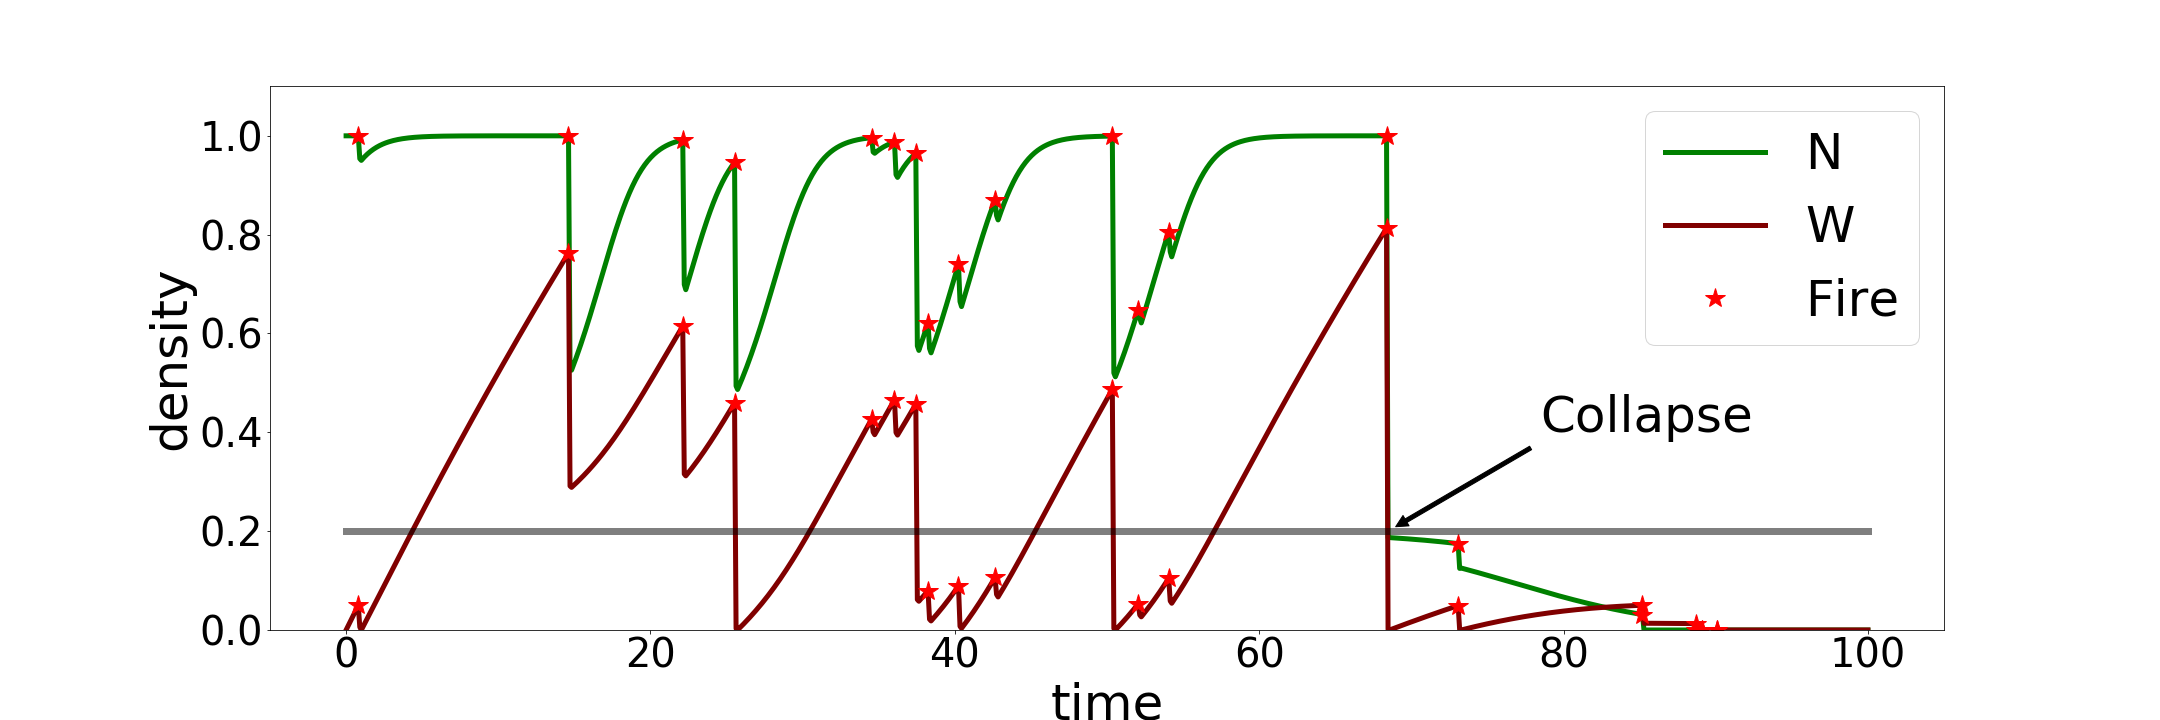
\includegraphics[width=12.cm]{time_series_cp_1.png}
\caption{Collapse}
%\label{fig:universe}
\end{figure}


\paragraph{}
Measuring collapse probability need to run several simulation to approximate it. However, it will depend on the time study used. Indeed, more the time study is long, the more is the risk to collapse. Even if it could be enough to used always the same time study, we present an improvement of this measure : probability to collapse by time unit. This upgrade is thus independent of the time study choose (details in \hyperref[proba_per_time_unit]{appendix}).



\paragraph{}
Another measure of the system is variability. It could be useful to consider variability because forest management traditionally tends to lock the variability \cite{bergeron_natural_2002} of the biomass. Another argument is that variability could be used to predict a critical change in the system, here a collapse, \cite{karr_population_1982} \cite{pimm_risk_1988} \cite{bengtsson_predicting_1995}. However other studies have shown no results \cite{bengtsson_interspecific_1989} \cite{pollard_extinction_1992} or a negative relationship \cite{lima_extinction_1996}.



\paragraph{}
Variability is defined like the variance when a collapse has not occur yet. Indeed, a collapse of the system will induce a bias in the computation of variability.


\begin{figure}[h!]
\centering
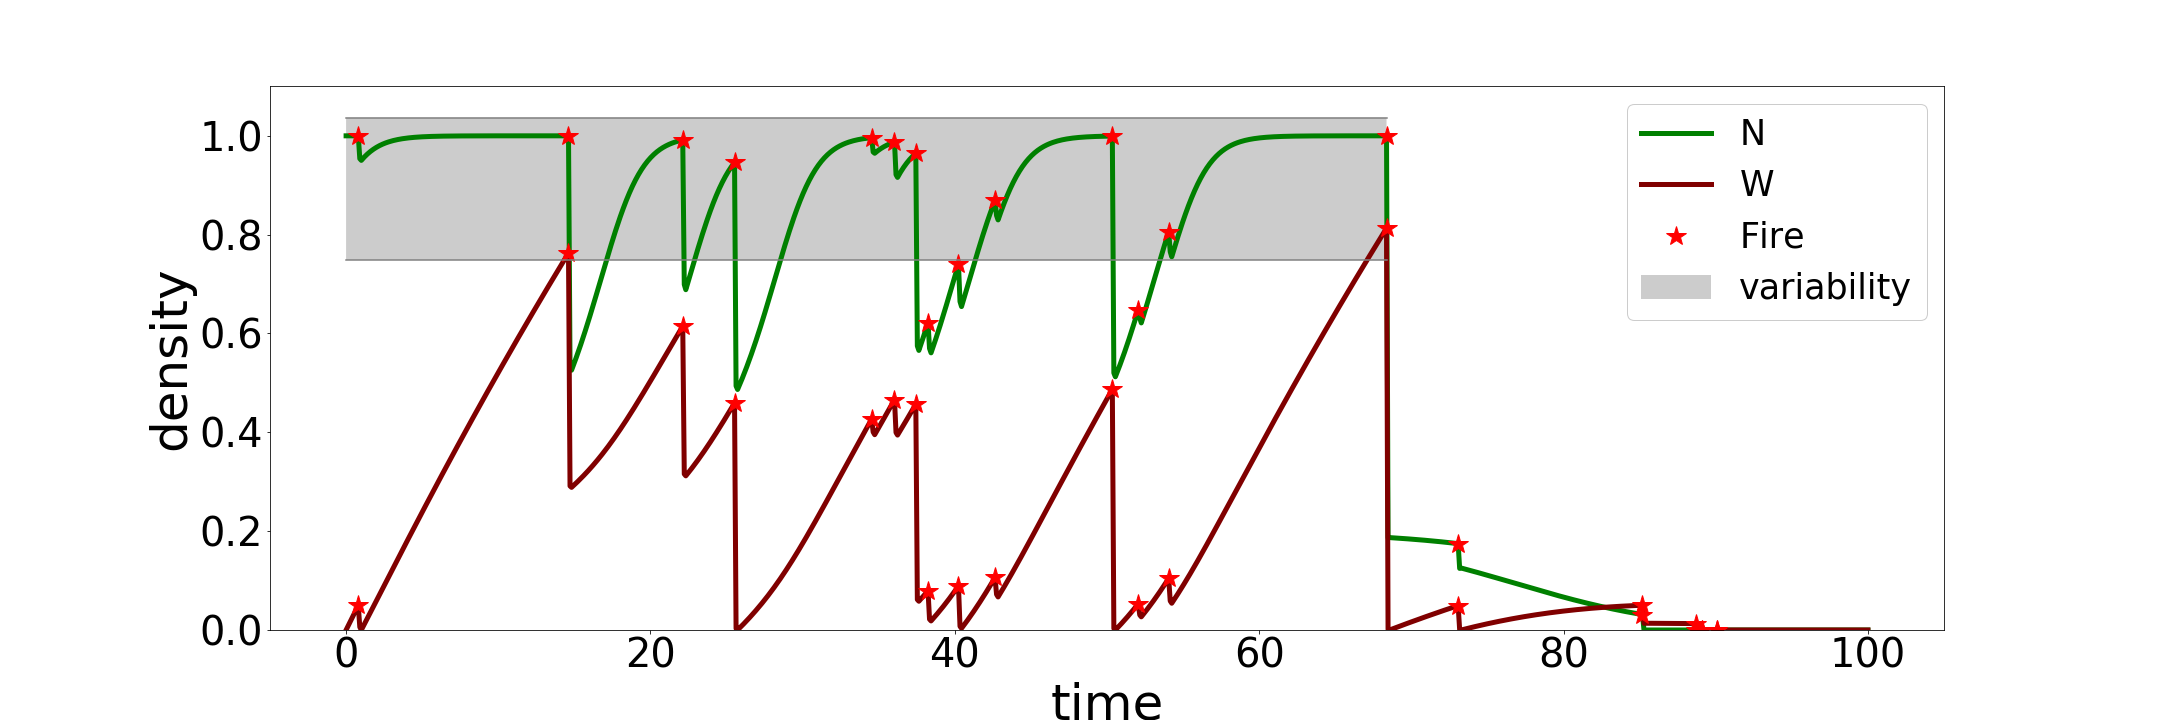
\includegraphics[width=12.cm]{time_series_sd_1.png}
\caption{Variability}
%\label{fig:universe}
\end{figure}



\paragraph{}
In practice, we have to make compromise to decrease different bias. Even if the dynamics is initialise close to the average approximation, it is safer to not take into account the first time of the time series to compute collapse probability (thus we do not consider the first $10\%$ of the time series). Also, as explain previously, it make no sens to compute variability after a collapse occurs, but in order to use the same time to measure variability, we restrict at the second $10\%$ of the time series. Indeed, the bias of time series not used because they collapse to soon is here quite low (\hyperref[algo_variability]{algorithm in appendix}). Other way to measure variability have been implemented and could be found in \hyperref[other_variability]{appendix}.


\begin{figure}[h!]
\centering
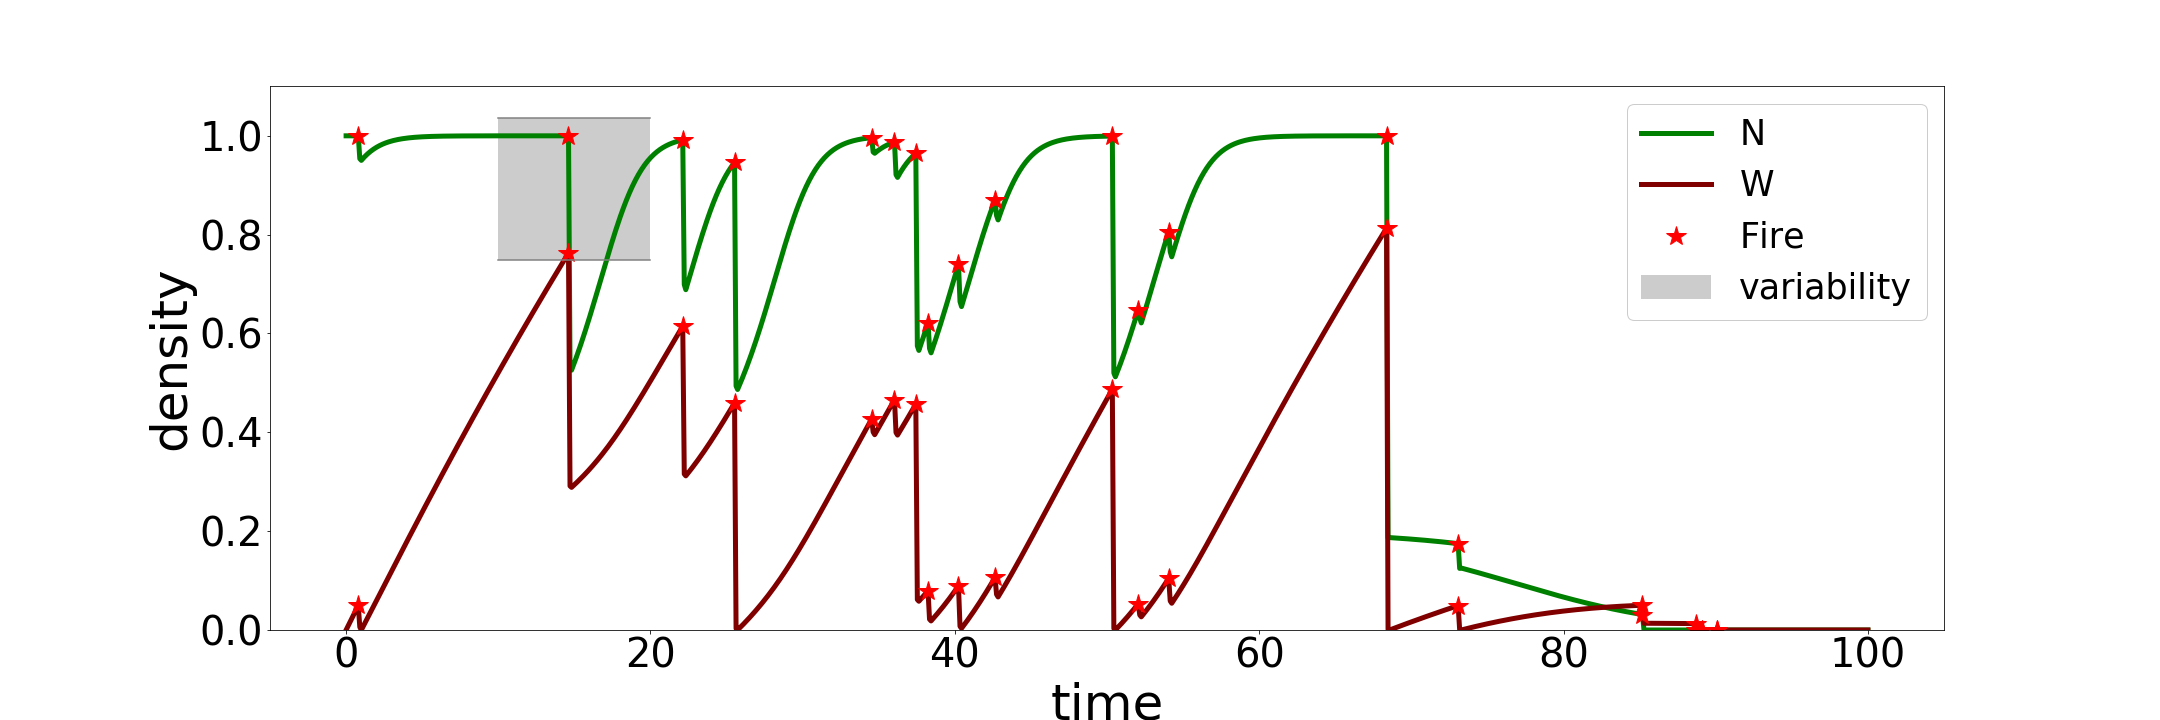
\includegraphics[width=12.cm]{time_series_sd_2.png}
\caption{More robust variability}
%\label{fig:universe}
\end{figure}


\paragraph{}
A similar measure to variability is the coefficient of variability. Defined as the variability over the mean. Indeed, a good measure of variability will be independent of the mean abundance if the dynamics are the same, but will not be independent if the dynamics change with mean abundance \cite{gaston_measurement_1993}\cite{noauthor_temporal_1994}







\paragraph{}
Different technique have been used to minimise the bias to variability estimation, due to collapse. However the bias persist \cite{seely2004complex}, that is why instead of doing a lot of simulation and average the effect, we propose to used only one simulation (only one fire). One problem is that when we change the frequency, we need to choose between used the same time scale, and so not take the same fire (it will truncated) or used the same fire and so no have the same time scale. Because both are relevant, both are computed. 


%Variability analysis should be performed on data that are free from artefact \cite{seely2004complex} 

%\todo{More time means more variation \cite{lawton1988more} }


\begin{figure}[h!]
\centering
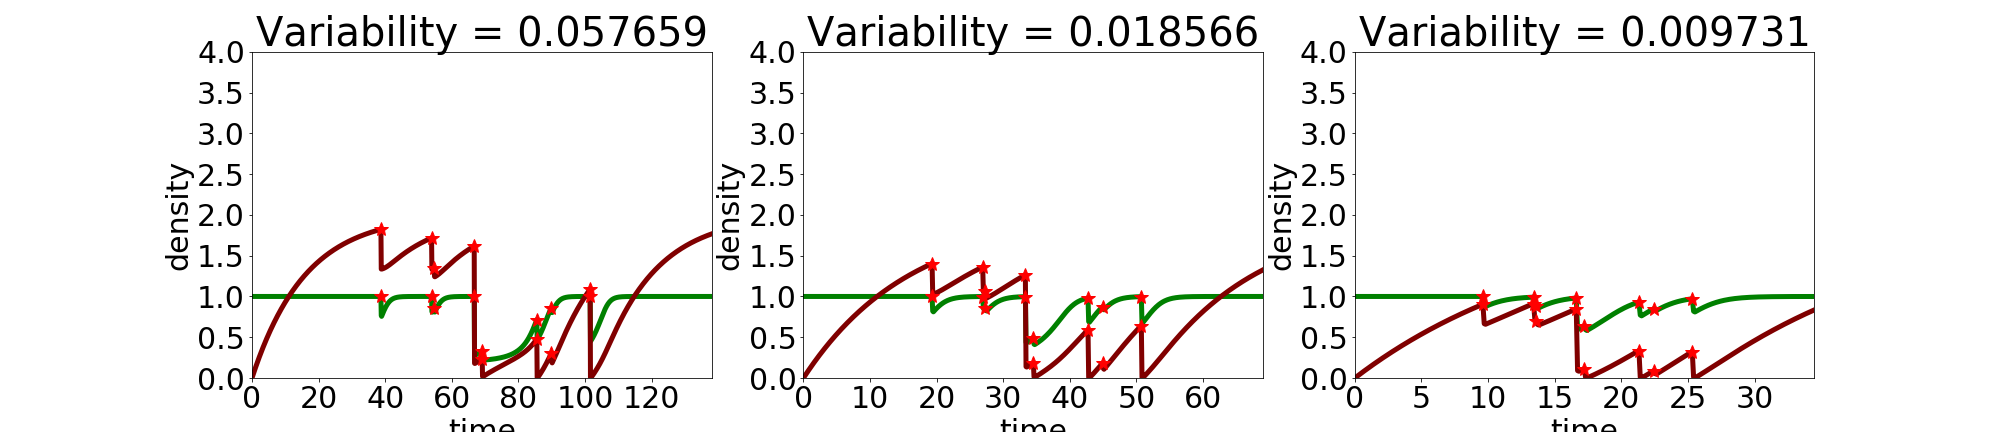
\includegraphics[width=12.cm]{same_2.png}
\caption{Same fire randomisation for different frequency and final time corresponding}
%\label{fig:universe}
\end{figure}

\begin{figure}[h!]
\centering
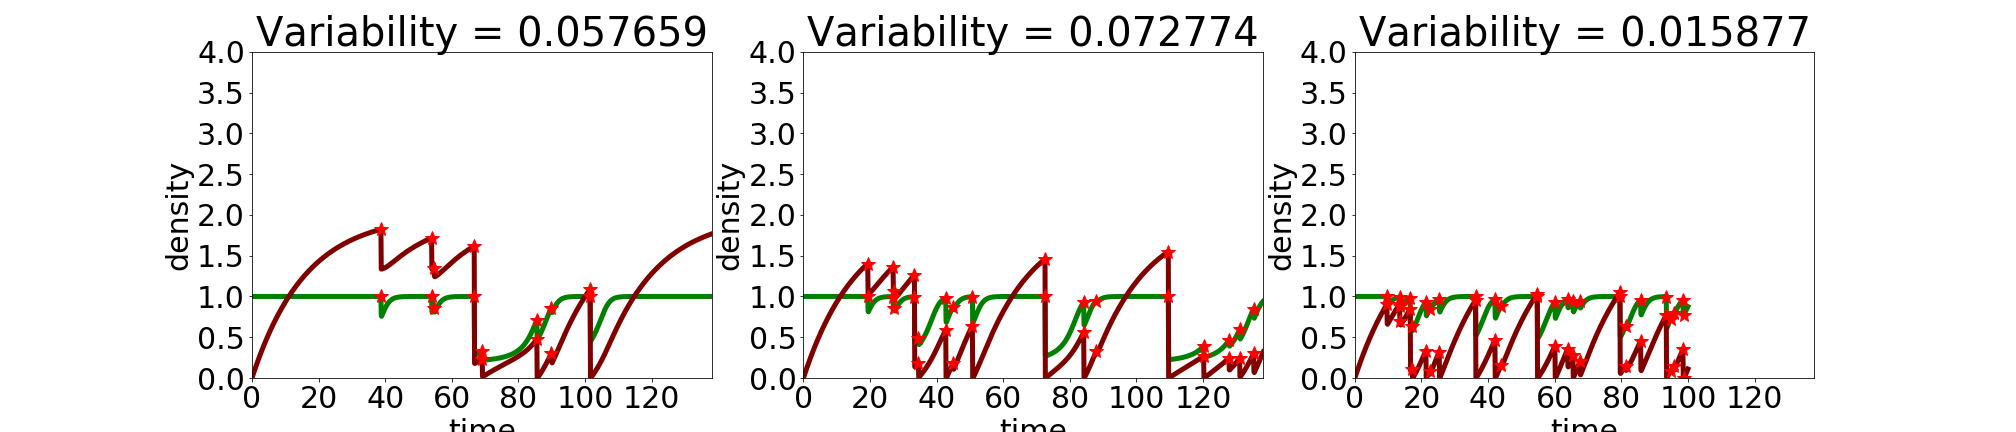
\includegraphics[width=12.cm]{same_1.png}
\caption{Same fire randomisation for different frequency and same final time (the first fire are the same, but the last are not necessarily present)}
%\label{fig:universe}
\end{figure}



\subsubsection{Estimation}


\paragraph{} % estiamtion
Numerical approximation of measures have two main drawback. Firstly, lot of time is needed, especially if we want to have a robust approximation (and so used long time simulation) and / or if we want to compute measure on a lot of parameters sets. Also, numerical approximation of measures do not give direct information of which and how parameters affect the measures. 
Thus, both collapse probability and variability are analytically estimated.

\paragraph{} % estimation variability
The estimation of variability is based on the assumption that the two density $N$ and $W$ remain close to their \hyperref[average_estimation]{average estimated} by $N^{av}$ and $W^{av}$. 

We denote $\lambda$ the average severity of a fire, estimated by
\[
\lambda = min(\{s(N^*+\alpha W^*), \frac{W^*}{\beta s (N^*+\alpha W^*)}\})
\]
We make the assumption that the effect of fire are independent (which is true when the dynamics is close to linear).
And so, we predict the variability with, \cite{zelnik_impact_2018}
\[
variability = f\frac{\lambda^2}{U}
\]
Details in \hyperref[variability_estimation]{appendix}


\todo{figure for just this estimation of variability}
\begin{figure}[h!]
\centering
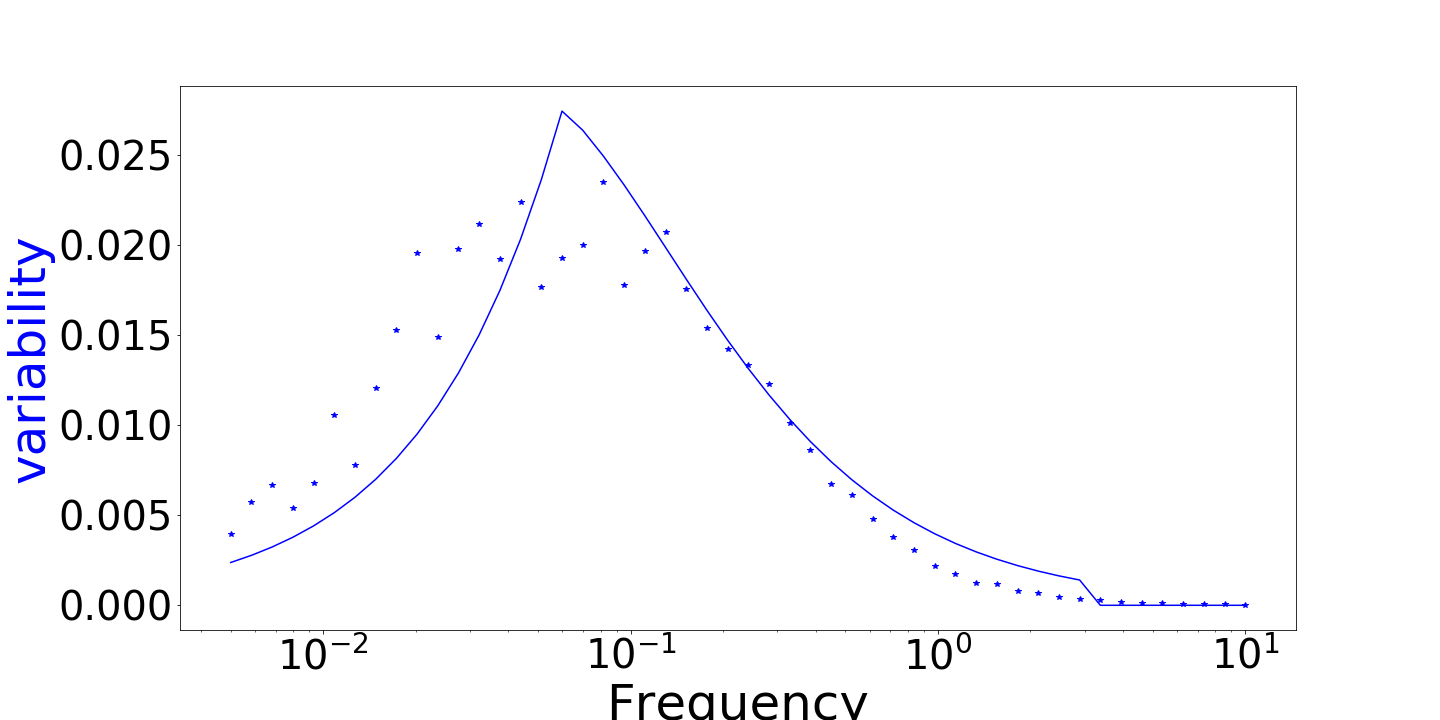
\includegraphics[width=10.cm]{variability_good.png}
\caption{Variability estimation}
%\label{fig:universe}
\end{figure}

\paragraph{}
Of course, the precision of this estimation depend greatly to the parameters region. For example, on the figure below, we can see that the approximation is less accurate. We can see ... \todo{depend on the plot ... describe what is the difference}

Generally, when the total severity of the fire is high, the accuracy of the estimation decreases. In practice, the product of the parameter $s.\alpha.\beta$ give an interesting clue of the precision of the variability estimation.

Other estimation of variability have been implement and are presented in \hyperref[variability_estimation_other]{annexes}.

\todo{make agian the plot with just the used estimation (just the "good" ones)}
\begin{figure}[h!]
\centering
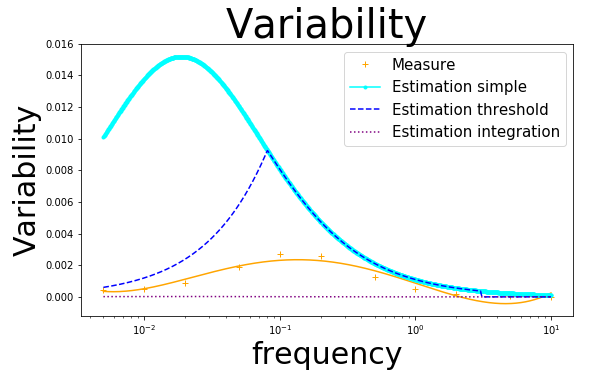
\includegraphics[width=10.cm]{variability_2.png}
\caption{Variability estimation}
%\label{fig:universe}
\end{figure}


\paragraph{}
Same as variability, we also estimate the collapse probability.

For this, we assume that the system can only collapse with a unique fire. This probability is called $cp1$. Derivation could be found \hyperref[cp_derivation]{appendix}
\[
\begin{array}{rcl}
cp1 & = & (N^*+\alpha W^*)((N^*-a+s)\exp(-\frac{N^*-a}{s}) - (\frac{W^*}{\beta}+s)\exp(-\frac{W^*}{s\beta})
\end{array}
\]
This probability is considered to follow a binomial law.
\[
\begin{array}{rcl}
cp & = & 1-(1-cp1)^{fT} \\
\end{array}
\]

\paragraph{}
Here again, the estimation work generally quite well, but the correctness dependent greatly on the set of parameter.

More generally, even if the maximum of the collapse probability is under estimated, the location of the peak is quite well predicted. As previously, the biases increase with the severity of the fire.


\todo{do again the plot with a the left work well, and not very well for the right.}
\begin{figure}[h!]
\centering
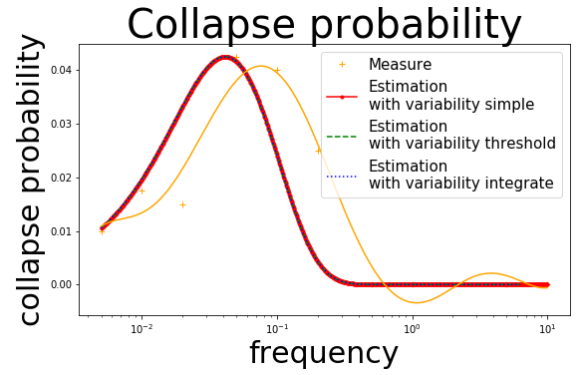
\includegraphics[width=6.cm]{cp.png}
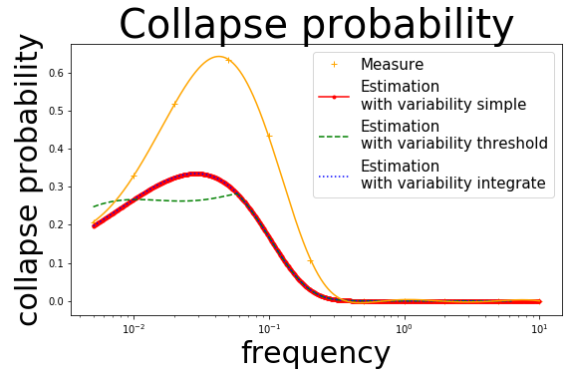
\includegraphics[width=6.cm]{cp_threshold.png}
\caption{Cp estimation}
%\label{fig:universe}
\end{figure}



\paragraph{}
In this study, we focus on two measures : variability and collapse probability. However as details in the introduction, several different notion of \hyperref[stability_litterature]{stability} are established. This different aspect of stability are briefly presented in  \hyperref[stability_others]{appendix}.




\subsection{Classification of dynamical behaviour}

\label{axes_definition}

\paragraph{}
The aim of this section is to give two axes, to grade a dynamical behaviour, given the corresponding set of parameters.


\subsubsection{Fuel accumulation versus depletion}

\paragraph{}
The first axes focuses on representing the major effect between accumulation of fuel and fuel burning. In order to do this, we approximate the average of each effects at the point $(1, \frac{m}{2d})$. The approximation $N=1$ is reasonable because $N$ is usually close to $1$. We make the derivation when $W = \frac{m}{2d}$ because we can see if at this point the dynamics tends to pull back fuel at a lower level or at a higher level. For example, if for a set of parameter, fuel accumulation dominate, the fuel is usually higher than $W = \frac{m}{2d}$ and if this density go down at this point the dynamics will tends to increase the level of fuel.
%\todo{perhaps come back at the choice of "initial point" at he of demonstration to justify why it make sense}

\paragraph{}
Firstly, we want to estimate the fuel accumulation rate at the point $(1, \frac{m}{2d})$. We rewrite the second equation of the system without the fire term (we denote $W_g$ the solution of this new equation).
\[
\left\lbrace
\begin{array}{rcl}
\frac{d W_g}{dt} & = & mN-dW_g \\
W_g(0) & = & \frac{m}{2d} \\
\end{array}
\right.
\]
The solution is,
\[
\begin{array}{rcl}
W_g(t) & = & \frac{m}{d}(1-\frac{1}{2}\exp(-td)) \\
\end{array}
\]
And the fuel accumulation rate (at the point $(1, \frac{m}{2d})$) is 
\[
\begin{array}{rcl}
\frac{dW_g}{dt}|_{t=0} & = & \frac{m}{2} \\
\end{array}
\]
The fuel accumulation rate is $\frac{m}{2}$.


\paragraph{}
We want now to approximate the fuel burning rate of $W$. The general fire term is 
\[
\delta_f(t)s(t)\beta(N+\alphaW)
\]
Applied at the point $(1, \frac{m}{2d})$ it is,
\[
\delta_f(t)s(t)\beta(1+\alpha\frac{m}{2d})
\]
We average the stochastic effect and have
\[
fs\beta(1+\alpha\frac{m}{2d})
\]
The average fuel burning rate is $fs\beta(1+\alpha\frac{m}{2d})$.

\paragraph{}
We can now define the first axes like the ratio of the fuel \textit{Accumulation} rate over the average fuel \textit{Burning} rate.

\[
\begin{array}{rcl}
AB & = & \frac{fs\beta(1+\alpha\frac{m}{2d})}{\frac{m}{2}} \\
AB & = & fs\beta(\frac{2}{m}+\frac{\alpha}{d}) \\
\end{array}
\]


\subsubsection{Possibility to collapse}


\paragraph{}
The second axis represent the possibility to collapse. Indeed, it is unlikely collapse if the severity of the fire is really low (compare to $N = 1$). We can define the axis 
%We say that the system is unlikely collapse if the probability to collapse with only one fire is lower than $0.01$.
\[
\begin{array}{rccl}
                &  P(s(N+\alpha W) > N-a ) & < & 0.01 \\
\Leftrightarrow &  P(s(1+\alpha \frac{m}{d}) > 1-a ) & < & 0.01 \\ 
\Leftrightarrow &  P(s > \frac{1-a}{(1+\alpha \frac{m}{d})} ) & < & 0.01 \\ 
\Leftrightarrow &  \exp(-\frac{1-a}{s(1+\alpha\frac{m}{d})}) & < & 0.01 \\ 
\end{array}
\]




\paragraph{}
Also, for some set of parameter, it is impossible to collapse because they are never enough fuel to maintain a fire strong enough to collapse the forest. We will place this particular specimen at the beginning of the axis.

%We now consider the equilibrium point $(1, \frac{m}{d}$) because it is when both $N$ and $W$ are higher and thus the total severity of the fire is higher too.

We still consider to be close to the equilibrium point $(1, \frac{m}{d}$).
\[
\left\lbrace
\begin{array}{rcl}
     N & = & 1 \\
     W & = & \frac{m}{d} \\
\end{array}
\right.
\]
Thus, the quantity burned in only one fire can not be higher than $\frac{m}{d}$. \\
Formally,
\[
\begin{array}{crcl}
&s\beta(N+\alpha W) & < & W \\
\Rightarrow & s\beta(1+\alpha \frac{m}{d}) & < & \frac{m}{d} \\
\end{array}
\]
For the first equation (for $N$) we have a collapse only if
\[
\begin{array}{rccl}
                &  s(N+\alpha W) & > & N-a \\
\Leftrightarrow &  s(1+\alpha \frac{m}{d}) & > & 1-a \\ 
\Leftrightarrow &  \frac{m}{d\beta} & > & 1-a \\ 
\Leftrightarrow &  \frac{m}{d( 1-a)} & > & \beta \\ 
\end{array}
\]
Thus, if this condition is not respected (in practice when $\beta$ is high enough) it is impossible to have a collapse. We can see below  an example when the lack of $W$ prevent the collapse of the forest.

\begin{figure}[h!]
\centering
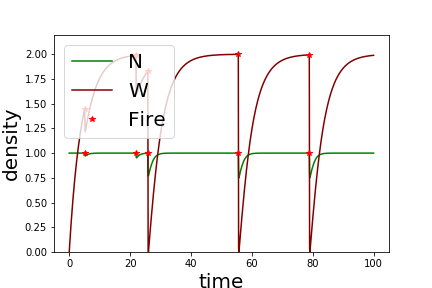
\includegraphics[width=12cm]{return_never_1.png}
\caption{For this set of parameter, even for a strong fire, fuel is too low to maintain a fire able to collapse the system}
%\label{fig:universe}
\end{figure}

\paragraph{}
In conclusion, the second axis is constructed by the severity of the fire compared to others parameters, 
\[
\exp(-\frac{1-a}{s(1+\alpha\frac{m}{d})})
\]
and for some specimen when the fuel is not enough to maintain a fire, when the following expression is not respected,
\[
\frac{m}{d( 1-a)} > \beta
\]
the specimen is constrained to be at the lower level of the axis.


\newpage
%%%%%%%%%%%%%%%%%%%%%%%%%%%%%%%%%%%%%%%%%%%%%%%%%%%%%%%%%%%%%%%%%%%%%%%%%%%%%%%%%%%%%%%%%%%%%%%%%%%%%%%%%%%%%%%%%%
% Result
%%%%%%%%%%%%%%%%%%%%%%%%%%%%%%%%%%%%%%%%%%%%%%%%%%%%%%%%%%%%%%%%%%%%%%%%%%%%%%%%%%%%%%%%%%%%%%%%%%%%%%%%%%%%%%%%%%

\section{Results}

\subsection{Model dynamics}


%a= 0.02 , m= 0.25 , d= 0.015625 , strength= 0.005 , alpha= 20 , beta= 2.0 % linear
%a= 0.02 , m= 0.25 , d= 0.015625 , strength= 0.01 , alpha= 40 , beta= 2.0 % counter
%a= 0.02 , m= 0.5 , d= 0.015625 , strength= 0.01 , alpha= 10 , beta= 2.0 % clock

\paragraph{}
We being by considering the possible dynamics that can occur in our model. Here, by changing only the value of $d$, in particular, the frequency remain the same, we have three time series with different general behaviour.

In the first one, the recovery after a fire is slow and the level of fuel is usually high which allow the system to collapse. For another example, the recovery is still slow, however, the level of fuel remain lower thus the system can resist to collapse. In the last illustration, the recovery is fast, and because the level of fuel is too low, a fire could not collapse the system.

By changing only one parameter, we have different dynamical behaviour, and different consequences for variability and collapse probability.

\begin{figure}[h!]
\begin{center}
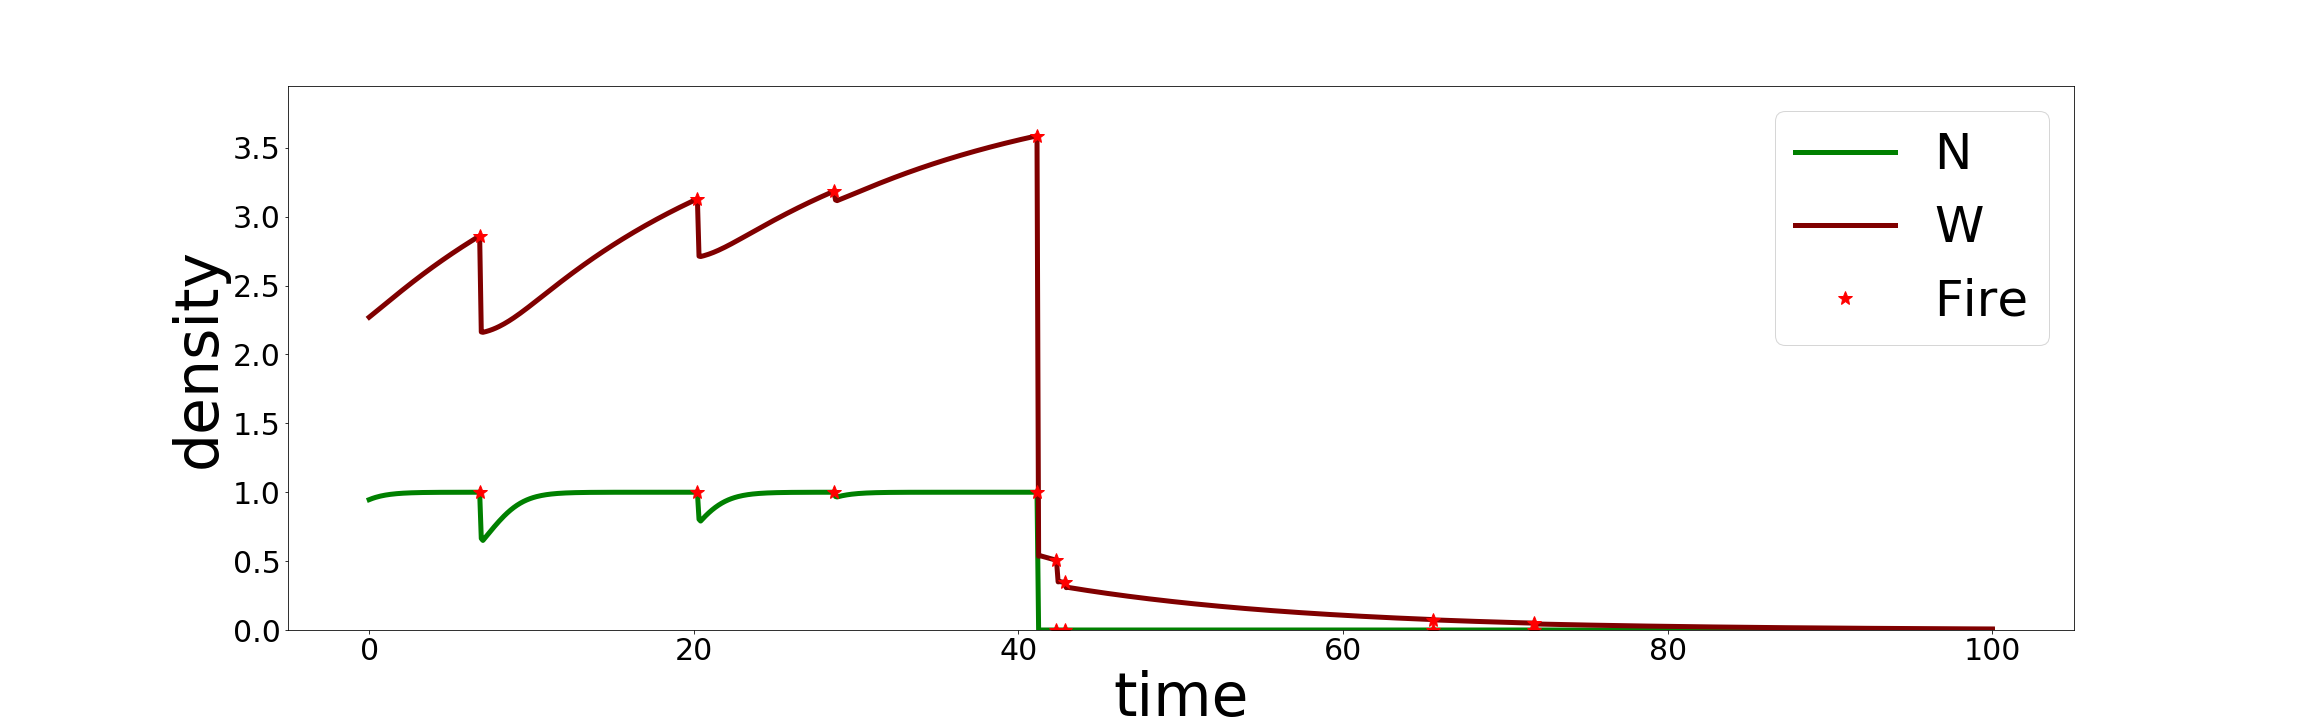
\includegraphics[height = 3.8cm]{results/time_series_2.png}
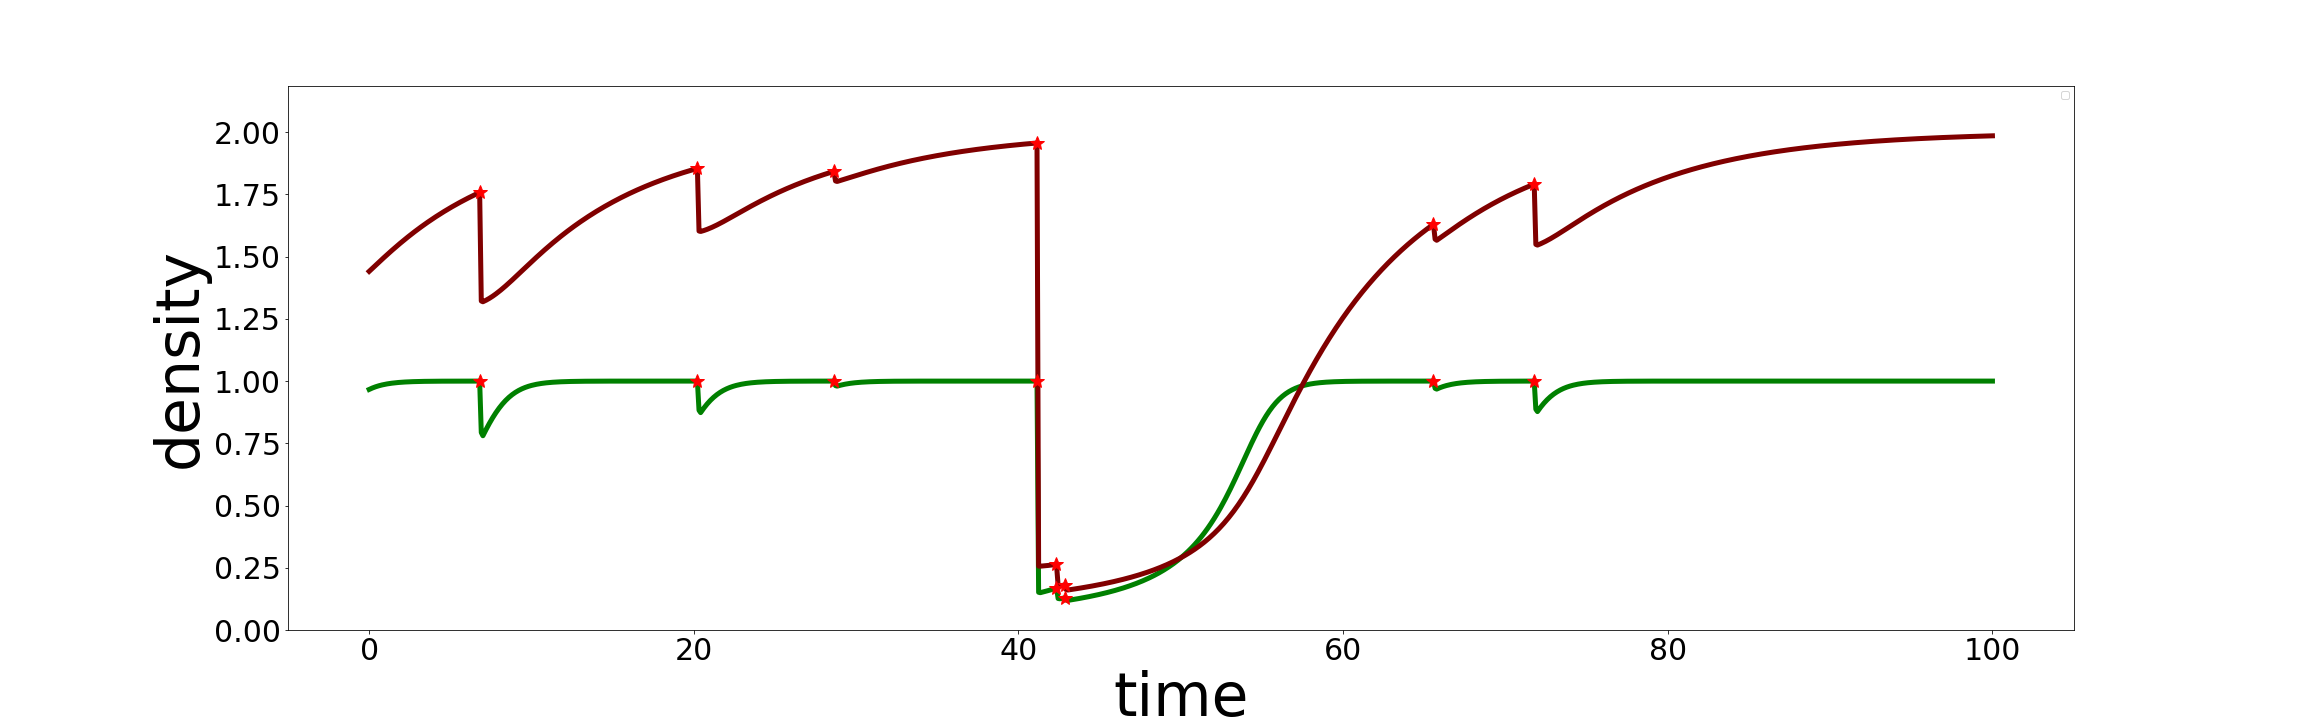
\includegraphics[height = 3.8cm]{results/time_series_3.png}
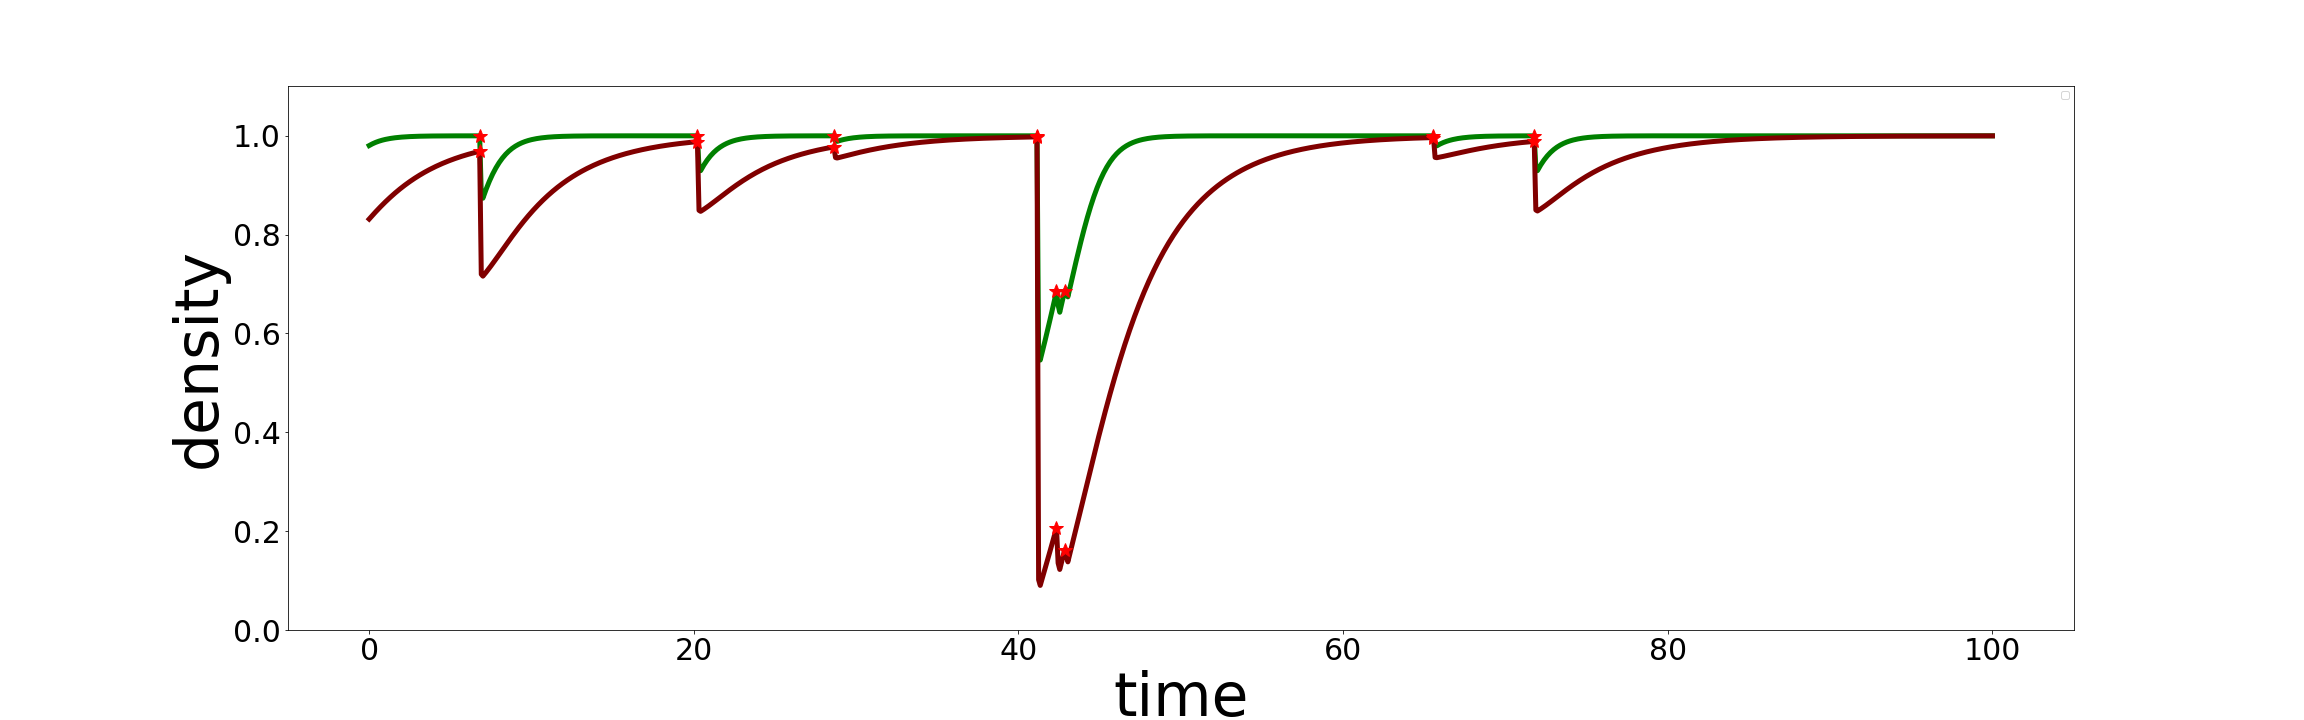
\includegraphics[height = 3.8cm]{results/time_series_4.png}
\end{center}
\caption{\label{fig:temp}Time series with different values of $d$ : $0.0625$, $0.125$ and $0.25$}
\end{figure}
% or category or type, kinds 
% Time series for three different value of $m$ and $\alpha$
% the general behaviour is different ...
%Class linear, counter-clockwise and clockwise



\newpage

\subsection{Dynamics cases}

%\paragraph{}
%In order to better understand the dynamics of the system, we distinguish different cases (and later subcases). Indeed, this facilitate the study, because we can so study case by case the different dynamics and their respective consequences.

%\paragraph{}
%A better differentiation could be done, it is possible to determine different cases of typical dynamical behaviour.
%%\paragraph{}
%Because we want to explore exhaustively the different dynamics cases, we introduce a coefficient to distinguish typical cases. Different \hyperref[other_ratio]{others coefficients} have been tested but only the following is used. After, another axes will be used to subdivide each cases.

\paragraph{}
Although we see different behaviour by changing only one parameters, the connection is not clear. So we will now try to clarify this by using \hyperref[axes_definition]{previously defined} axes by which we can exhaustively compare all the possible types of dynamics.
    
The first axes compare the effect of fuel decay and burning. The first axes is also used to construct the second one : the possibility to collapse.

Below are presented several time series for each subcases, in order to give an idea of the general behaviour for each cases.


\begin{figure}[h!]
\centering
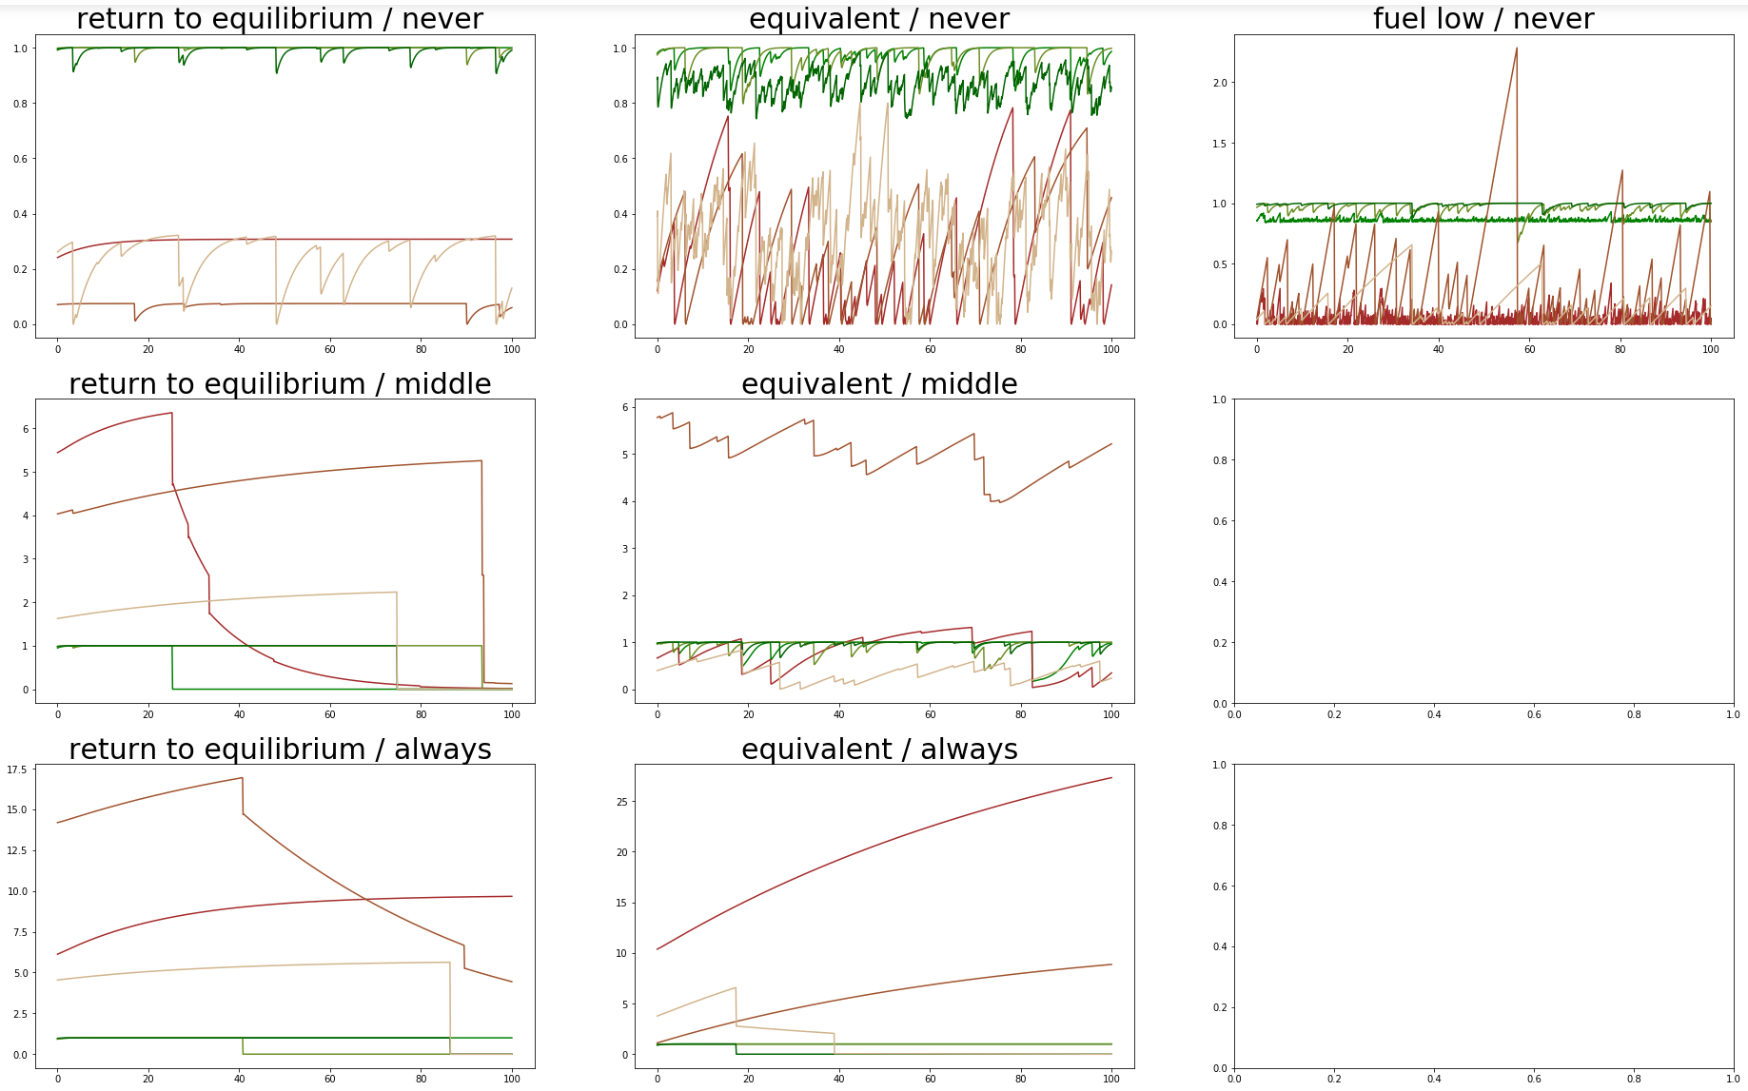
\includegraphics[width=12cm]{results/time_series_each_cases.png}
\caption{Typical dynamical cases along the two axes \textit{accumulation VS depletion} and \textit{possibility to collapse}}
%\label{fig:universe}
\end{figure}


\subsubsection{Accumulation VS depletion}

\paragraph{}
Indeed, the two previously defined axes could help to distinguish typical dynamical cases. We choose two separate the first axes in three part, by using two threshold ($0.5$ and $20$) for the value of the ratio \textit{AB}. The first part correspond to the cases when fuel accumulate a lot. In this case, fuel have usually time to come back at equilibrium ($W^{eq}=\frac{m}{d}$) before another fire occurs.

\begin{figure}[h!]
\centering
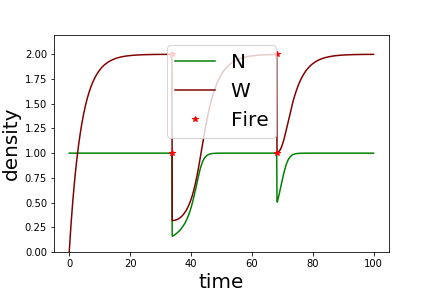
\includegraphics[width=3.9cm]{return_to_eq_1.png}
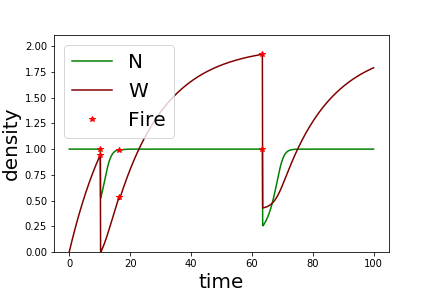
\includegraphics[width=3.9cm]{return_to_eq_2.png}
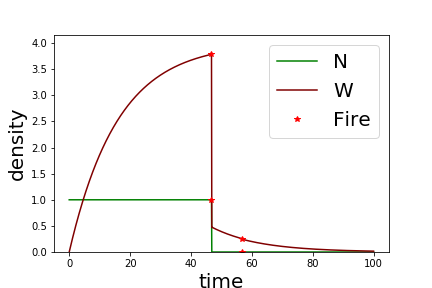
\includegraphics[width=3.9cm]{return_to_eq_3.png}
\caption{Time series for different parameter sets corresponding to the case : Return to equilibrium}
%\label{fig:universe}
\end{figure}



\paragraph{}
At the opposite, when the ratio called \textit{AB} is high, in another word when fire tend to annihilate the growth of $W$, this one remains low. 
\begin{figure}[h!]
\centering
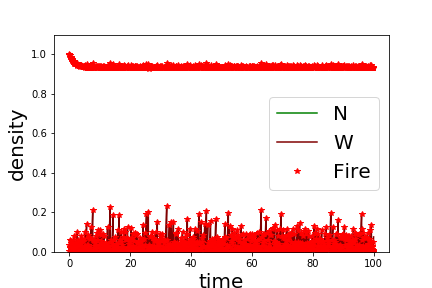
\includegraphics[width=3.9cm]{continue_1.png}
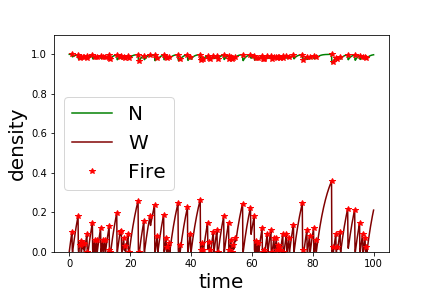
\includegraphics[width=3.9cm]{continue_2.png}
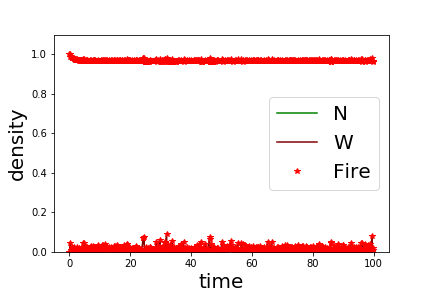
\includegraphics[width=3.9cm]{continue_3.png}
\caption{Time series for different parameter sets corresponding to the case : depletion}
%\label{fig:universe}
\end{figure}


\paragraph{}
Between the two previous cases, we define a third cases called \textit{fluctuation}. It happens when the effect of the fire and the growth are about the same quantity. In this case, $W$ can take the larger range of value (from $0$ to $W^{eq}=\frac{m}{d}$).
\begin{figure}[h!]
\centering
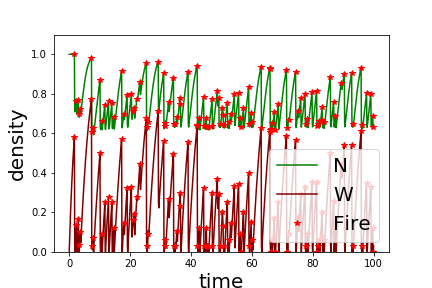
\includegraphics[width=3.9cm]{middle_1.png}
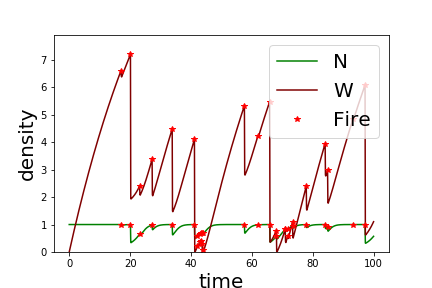
\includegraphics[width=3.9cm]{middle_2.png}
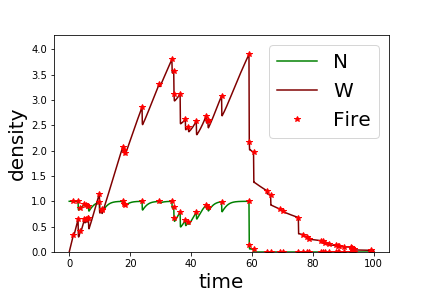
\includegraphics[width=3.9cm]{middle_3.png}
\caption{Time series for different parameter sets corresponding to the case : fluctuation}
%\label{fig:universe}
\end{figure}


\paragraph{}
In order to visualise the limit of each cases, examples for each limits are presented.
For the limit between \textit{accumulation} and \textit{fluctuation} we could see that a fire often occur before the dynamics come back to equilibrium. For the second one, we see that fuel is quite low, but could sometimes take relatively high value.


\begin{figure}[h!]
\centering
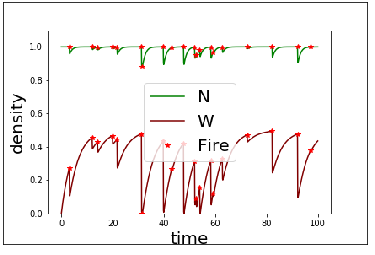
\includegraphics[width=3.9cm]{lim_eq_middle_1.png}
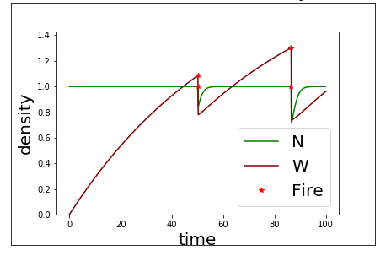
\includegraphics[width=3.9cm]{lim_eq_middle_2.png}
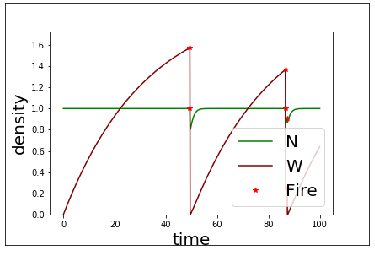
\includegraphics[width=3.9cm]{lim_eq_middle_3.png}
\caption{Time series for different parameter sets corresponding to the limit between accumulation and fluctuation}
%\label{fig:universe}
\end{figure}


\begin{figure}[h!]
\centering
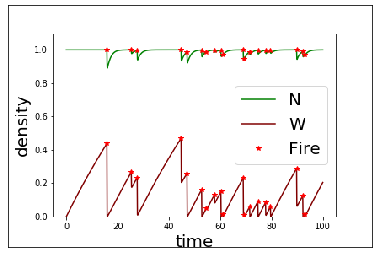
\includegraphics[width=3.9cm]{lim_c_middle_1.png}
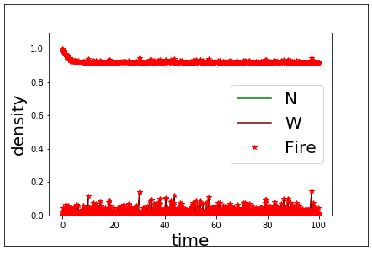
\includegraphics[width=3.9cm]{lim_c_middle_2.png}
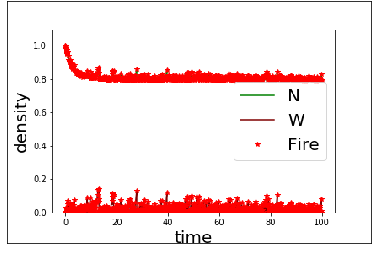
\includegraphics[width=3.9cm]{lim_c_middle_3.png}
\caption{Time series for different parameter sets corresponding to the limit between depletion and fluctuate}
%\label{fig:universe}
\end{figure}



%%%%%%%%%%%%%%%%%%%%%%%%%%%%%%%%%%%%% subcases %%%%%%%%%%%%%%%%%%%%%%%%%%%%%%%%%%%%%%%%%%%%%%%%%%

\newpage

%\subsubsection{"Accumulation"}
\subsubsection{Possibility to collapse}


\paragraph{} %\todo{expand ? it is the main paragraph of the subsubsection ... }
After using the axis \textit{AB} to distinguish several part, we used the axis \textit{possibility to collapse}. Usually, three part could be done, by using a threshold ($0.01$ and $0.2$) to the value of the axis. The first one, called \textit{unlikely collapse}, which comprise the lower value of the axis and the cases where the condition $\frac{m}{d( 1-a)} & > & \beta$ is not respected. The transitory case called "possible collapse" when the collapse is unpredictable. And, the \textit{inevitable collapse} when the system have a fire could easily collapse the system.

Using the two axis together allow to have a grid of typical dynamical cases. However, the number of this cases is $7$ and not $9$, because for the case $depletion$ in other words the ratio \textit{AB} is high, the level of fuel is too low to allow a fire to  the system. We have not the case \textit{depletion - possible collapse} and surely not \textit{depletion - inevitable collapse}. Nonetheless, let recall that even is the case \textit{unlikely collapse}, the system is still able to collapse, but the risk is very low.




\paragraph{accumulation - unlikely collapse\\}
Below are presented two times series, with two different set of parameter corresponding to the case \textit{accumulation - unlikely collapse}. The left instance correspond at the case where the system not collapse because the condition $\frac{m}{d( 1-a)} & > & \beta$ is not respected, it could be verified that even is fire are strong, the lack of fuel stop it, and the system survive. The right instance correspond at low severity of the fire, the dynamics have time to come back at equilibrium between two fires.


\begin{figure}[h!]
\centering
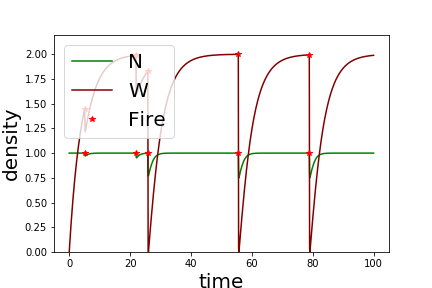
\includegraphics[width=6cm]{return_never_1.png}
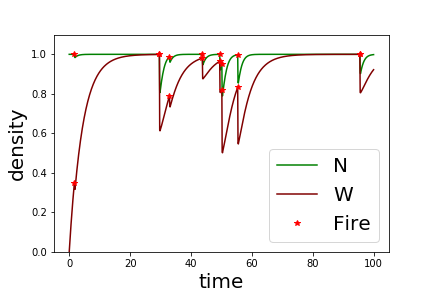
\includegraphics[width=6cm]{return_never_2.png}
\caption{Time series for different parameter sets corresponding to the case : Never collapse}
%\label{fig:universe}
\end{figure}


\paragraph{accumulation - inevitable collapse\\} % always
For some set of parameter, the system always collapse. Of course, it occurs, when the condition $\frac{m}{d( 1-a)} > \beta$ is respected. Also, the severity of the fire need to be strong enough to collapse. Because the family \textit{accumulation} implies that the dynamics usually return to equilibrium between two fires, the system could collapse only by a single and strong fire, as we can see below.

\begin{figure}[h!]
\centering
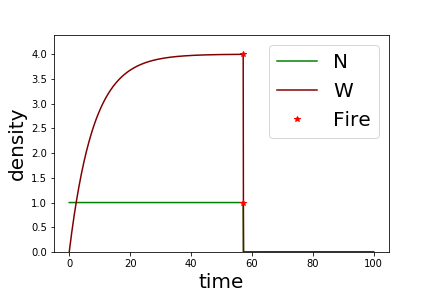
\includegraphics[width=3.9cm]{return_always_1.png}
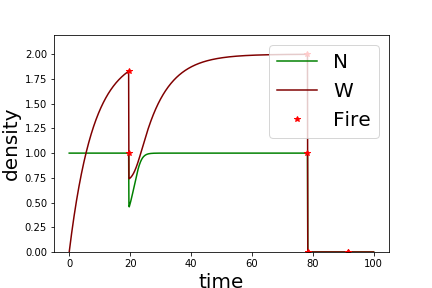
\includegraphics[width=3.9cm]{return_always_2.png}
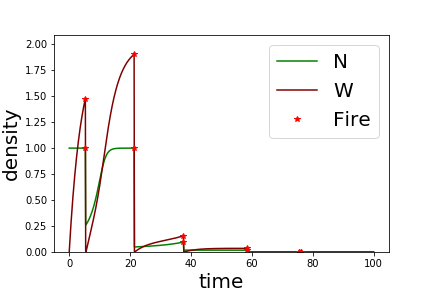
\includegraphics[width=3.9cm]{return_always_3.png}
\caption{Time series for different parameter sets corresponding to the case : accumulation - inevitable collapse}
%\label{fig:universe}
\end{figure}


%\todo{préciser que le temps d'étude n'est pas tjrs suffisant pour le constater}
\paragraph{accumulation - possible collapse \\} % between
Between this two extremes cases, exists a range of parameters when a collapse could occur. This happen, when $W$ is high enough and also when the actual strength of the fire is high enough. We could remark that this case depend greatly on the final time used, because this system are able to collapse, but need a strong enough fire. In other words, for a higher time study, the system would have more risk to collapse, because the probability to have a strong fire would be higher.


\begin{figure}[h!]
\centering
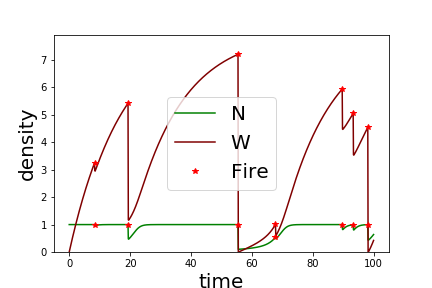
\includegraphics[width=3.9cm]{return_between_1.png}
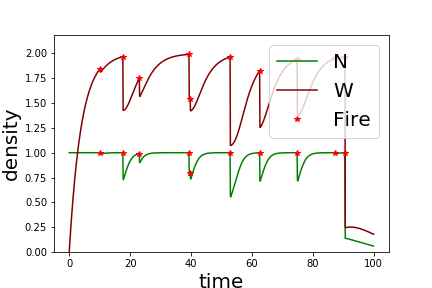
\includegraphics[width=3.9cm]{return_between_2.png}
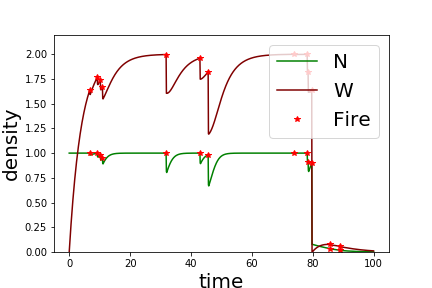
\includegraphics[width=3.9cm]{return_between_3.png}
\caption{Time series for different parameter sets corresponding to the case : accumulation - possible collapse}
%\label{fig:universe}
\end{figure}

%%%%%%%%%%%%%%%%%%  \todo{... link with cp (but after) ... } 

\paragraph{depletion \\}
Following the same idea than previously, when $W$ is always low, collapse can never occurs. In practice, we can observe a collapse only, when the set of parameter is closed to the case \textit{fluctuation}. So, $W$ can go higher enough to generate a fire. But this is observed rarely. On the figure below we can observe that $W$ come back to $0$ with each fire and have no time to accumulate to engender a strong fire.
%\todo{jamais collapse, expliquer pourquoi avec un très simple calcul}
%\todo{nuancer dans le cas ou on est proche du cas "equivalence" and fuel is not always low enough}

\begin{figure}[h!]
\centering
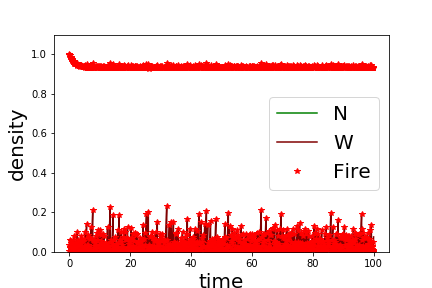
\includegraphics[width=6cm]{continue_1.png}
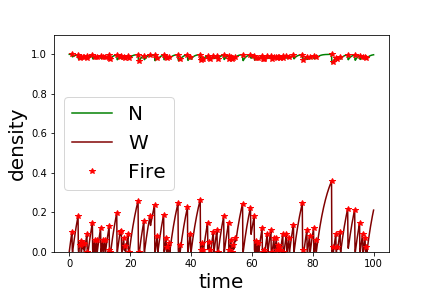
\includegraphics[width=6cm]{continue_2.png}
\caption{Time series for different parameter sets corresponding to the case : \textit{depletion}}
%\label{fig:universe}
\end{figure}



%\subsubsection{"fluctuating"}
%\todo{extrapoler, on divise en 2 cas pour s'approcher des 2 autres cas}
%\todo{quand proche continuous, collapse happen if fuel go too high}
%\todo{illustrate}

\newpage
\paragraph{fluctuating \\}
The case called \textit{fluctuating} is the harder to study, justly because $W$ fluctuates a lot, it is thus more difficult to have analytic results. Depending on the value of the ratio \textit{AB}, it could make sense to assimilate this case to the case \textit{accumulate} or \textit{depletion}.


\paragraph{}
When $AB$ is close enough to the limit with the case \textit{depletion}, we could consider that the level remain most of the time low enough to avoid collapse. However, the risk to collapse is here not negligible.


\begin{figure}[h!]
\centering
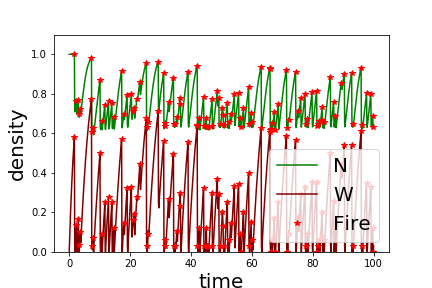
\includegraphics[width=5.5cm]{equivalent_high_1.png}
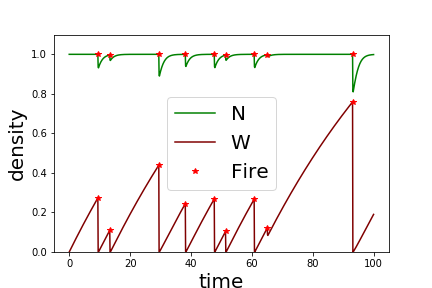
\includegraphics[width=5.5cm]{equivalent_high_3.png} \\
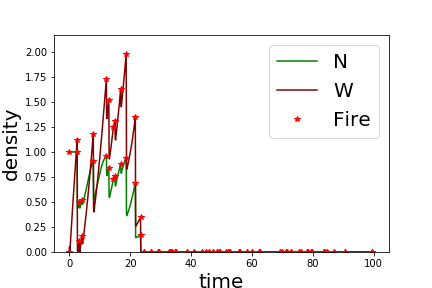
\includegraphics[width=5.5cm]{equivalent_high_2.png}
\caption{Time series for different parameter sets corresponding to the case : \textit{fluctuation}, but close to \textit{depletion}}
%\label{fig:universe}
\end{figure}

\newpage
\paragraph{}
Also, when $AB$ is lower, we have again the same three sub-cases than for the \textit{accumulation} case. We can observe that for this example, the dynamics do not change much.%, and that the extrapolation could make sense (but only if $AB$ is low enough).
%\todo{ratio low, proche "return", on herite des 3 cas, never always, between}
%\todo{illustrer 3 exemples pour chaque cas}

%\paragraph{}

\begin{figure}[h!]
\centering
\includegraphics[width=3.9cm]{equivalent_low_never_1.png}
\includegraphics[width=3.9cm]{equivalent_low_never_2.png}
\includegraphics[width=3.9cm]{equivalent_low_never_3.png}
\caption{Time series for different parameter sets corresponding to the case : fluctuating - unlikely collapse}
%\label{fig:universe}
\end{figure}


%\paragraph{}

\begin{figure}[h!]
\centering
\includegraphics[width=3.9cm]{equivalent_low_always_1.png}
\includegraphics[width=3.9cm]{equivalent_low_always_2.png}
\includegraphics[width=3.9cm]{equivalent_low_always_3.png}
\caption{Time series for different parameter sets corresponding to the case : fluctuating - possible collapse}
%\label{fig:universe}
\end{figure}



%\paragraph{}

\begin{figure}[h!]
\centering
\includegraphics[width=6cm]{equivalent_low_between_1.png}
\includegraphics[width=6cm]{equivalent_low_between_2.png}
\caption{Time series for different parameter sets corresponding to the case : fluctuating - inevitable}
%\label{fig:universe}
\end{figure}




\newpage
\subsection{Connection between variability and collapse probability}

\paragraph{}
One of our major focus is to study the impact of frequency over variability and collapse probability. We study this for each of the seven dynamical cases defined previously, with an appropriate range of value of frequency.

\paragraph{}
We begin with the dynamical case called \textit{accumulate - unlikely collapse}. The red font is used to mark the dynamical case \textit{accumulate} the yellow correspond to \textit{fluctuation}. We could see that the variability increase whit the frequency, however, collapse probability remains null. We can remark that the estimation (the continuous line) work reasonably well. 

\todo{do again the plot with good name, and ...}
\begin{figure}[h!]
\begin{center}
\includegraphics[width=10cm]{results/return_never_2.png}
\end{center}
\caption{\label{fig:temp}Measures evolution over frequency for the dynamical cases : accumulate - unlikely collapse}
\end{figure}


\paragraph{}
Here, the collapse probability is still null. The is firstly increasing, following the behaviour of the case \textit{accumulate - unlikely collapse} and decrease after, when we approaching the \textit{depletion} dynamical case.


\begin{figure}[h!]
\begin{center}
\includegraphics[width=10cm]{results/equivalent_never.png} \\
\end{center}
\caption{\label{fig:temp}Measures evolution over frequency for the dynamical cases : fluctuation - unlikely collapse}
\end{figure}


\paragraph{}
When frequency is high enough, $AB$ take high value, and the fuel is constrain to low value. The two measures are decreasing quickly. Depending on the parameter set, collapse probability could already be null, or crash in the depletion dynamical case.

\begin{figure}[h!]
\begin{center}
\includegraphics[width=10cm]{results/fuel_low.png}
\end{center}
\caption{\label{fig:temp}Measures evolution over frequency for the dynamical cases : depletion}
\end{figure}


\paragraph{}
For the two dynamical case \textit{accumulation - possible collapse} and \textit{accumulation - inevitable collapse} both variability and collapse probability are increasing.

To clarify, even in the dynamical case \textit{accumulation - inevitable collapse} the collapse probability could be low because they are not enough fire in the time study to have the risk to collapse the system.

\begin{figure}[h!]
\begin{center}
\includegraphics[width=6cm]{results/return_moderate_2.png}
\includegraphics[width=6cm]{results/return_always_2.png} 
\end{center}
\caption{\label{fig:temp}Measures evolution over frequency for the dynamical cases : Left \textit{accumulation - possible collapse}, Right \textit{accumulation - inevitable collapse}}
\end{figure}



\paragraph{}
For the two dynamical case \textit{fluctuation - possible collapse} and \textit{fluctuation - inevitable collapse} both variability and collapse probability are firstly increasing and after decreasing. 



\begin{figure}[h!]
\begin{center}
\includegraphics[width=6cm]{results/equivalent_moderate_2.png} \includegraphics[width=6cm]{results/equivalent_always.png}
\end{center}
\caption{\label{fig:temp}Measures evolution over frequency for the dynamical cases : Left \textit{fluctuation - possible collapse}, Right \textit{fluctuation - inevitable collapse}}
\end{figure}





\newpage

\paragraph{}
Inside each dynamical case, frequency affect both variability and collapse probability. Because $AD$ depend of frequency, changed this one could implies a changed of dynamical case. In order to study the effect of frequency across dynamical cases, we study the transition to one dynamical case to another one.

To do this, we compute the probability to change the dynamical case if the frequency is doubled. We have the following matrix transition.


%\paragraph{}
%Previously, the frequency range used was choose to remains in the same sub cases. Now, we want to know what happens when the frequency range is higher. To do this, we study the transition of subcases when we double the frequency. 

%We can see that the ability to collapse in one fire do not change, however, the ratio change, and thus, doubling the frequency could change the dynamical cases for axis 1 but not for axis 2. \todo{reformulate}


\begin{table}[h!]
    \centering
    \begin{tabular}{|c|c||c|c|c|c|c|c|c|}
        \hline
        $AB$ && \multicolumn{3}{c|}{accumulation} & \multicolumn{3}{c|}{fluctuation} & \\
        \hline
        & \rotatebox{45}{possibility to collapse} & \rotatebox{90}{unlikely collapse} & \rotatebox{90}{possible collapse} & \rotatebox{90}{inevitable collapse} & \rotatebox{90}{unlikely collapse} & \rotatebox{90}{possible collapse} & \rotatebox{90}{unlikely collapse} & \rotatebox{90}{depletion} \\
        \hline
        \hline
        \multirow{3}*{accumulation} & unlikely collapse & 0.757 & 0 & 0 & 0.243 & 0 & 0 & 0 \\
        \cline{2-9}
        & possible collapse & 0 & 0.167 & 0 & 0 & 0.833 & 0 & 0 \\
        \cline{2-9}
        & inevitable collapse & 0 & 0 & 0.743 & 0 & 0 & 0.257 & 0 \\
        \hline
        \multirow{3}*{fluctuation} & unlikely collapse & 0 & 0 & 0 & 0.838 & 0 & 0 & 0.162 \\
        \cline{2-9}
        & possible collapse & 0 & 0 & 0 & 0 & 0.857 & 0 & 0.143 \\
        \cline{2-9}
        & unlikely collapse & 0 & 0 & 0 & 0 & 0 & 0.827 & 0.173 \\
        \hline
        depletion && 0 & 0 & 0 & 0 & 0 & 0 & 1 \\
        \hline
    \end{tabular}
    \caption{Transition matrix}
%    \label{tab:my_label}
\end{table}




\paragraph{}
Now, the frequency ranged used is consequently higher. We focus on the general effect of changing frequency to the two measures. We could check below that for the extremes (low value of frequency and high value of frequency) both measures are very small, and they are higher for an intermediate value of frequency.


\paragraph{}
Depending on the parameter set choose, the dynamics is different and therefore, the variability and the collapse probability do not react similarly. On the first one, variability and cp first increase together and after decrease (the decreasing part is not always present). On the second one, the two measure are also increasing and decreasing but not in the same time, more surprisingly cp increase before variability. However, in the last class presented, the loop is clockwise.
\todo{another plot, with a counter clockwise more circular ?}


\begin{figure}[h!]
\begin{center}
\includegraphics[width=10cm, height = 4.2cm]{case_linear.png}
\includegraphics[width=10cm, height = 4.2cm]{case_triangular.png}
\includegraphics[width=10cm, height = 4.2cm]{case_clockwise.png}
\end{center}
\caption{\label{fig:temp}From left to right : Class linear, counter-clockwise and clockwise} % or category or type, kinds
\end{figure}



\todo{plot in results the graph with var and cp increasing with same fire and same time, to validate the results.}




\newpage
\subsection{Implication for perturbations effects.}


\subsubsection{fuel removal}

\paragraph{}
Now, we want to study the impact of the parameter $d$ to the variability and collapse probability of the system. To do this, we repeat the study for the three main "dynamical cases". Indeed, the second axes used to subdivide each cases use the notion of "collapse probability", which it make more sense here to measures it than to estimate it. 

In practice, we choose for each case a set of parameter in order to have be able to varies the value of $d$ while remaining in the same dynamic cases.

We can see that for each dynamics cases, increase $d$ decrease variability and collapse probability. This make sense, because increasing $d$ decrease the value of the $W^*$ the average of $W$. In practise it is clearly intuitive, if the decay of the dead wood is higher, the density of the dead wood tend to be lower. The consequences is that the fire have not anymore enough fuel to trigger a collapse and the variability is lower because $W$ take always small value.

However, if in the case "AB" variability and collapse probability are similar, for the case "fluctuating" variability decrease slower and after collapse probability. Also, in the case "fuel low", the variability decrease even if the collapse probability remains null.



\begin{figure}[h]
\begin{center}
\includegraphics[width=6cm]{results/return_to_equilibrium_1.png}
\includegraphics[width=6cm]{results/equivalent_1.png}
\includegraphics[width=6cm]{results/fuel_low_1.png}
\end{center}
\caption{\label{fig:temp}Impact of $d$, from left to right : "return to equilibrium, "fluctuating" and "fuel low"}
\end{figure}





\newpage
\subsubsection{Drought}


\paragraph{}
We now focus on the drought scenarios. This is a current subject (a lot of recent papers about this). This is mainly a consequence of extreme weather as a result of climate changed. It have been shown that drought increase the frequency, the severity and the size of fire. We link this scenarios to the parameters $f, s, \alpha$ and $\beta$ of our model. Also, because fuel are drier, parameters $\alpha$ and $\beta$ are higher. In brief, the consequences of climate warming is formalised by a higher values of both $f, s, \alpha$ and $\beta$.



\paragraph{}
It can be \hyperref[drought_increase]{demonstrated} that increasing this $4$ parameters increase the ratio $AB$. Thus, a drought scenarios will tend firstly to increase both variability and the collapse probability and after a decrease of both measures.

\todo{explain what we see below}
\paragraph{}


\todo{refaire plot sans estimation, en s'arretant aux limites et pas plus loin}
\todo{ET REFORMULER}

\begin{figure}[h]
\begin{center}
\includegraphics[width=6cm]{results/drought/return_never.png}
\includegraphics[width=6cm]{results/drought/equivalent_never.png}
\end{center}
\caption{\label{fig:temp}Left : return to equilibrium / never, Right : equivalent / never}
\end{figure}

\begin{figure}[h]
\begin{center}
\includegraphics[width=6cm]{results/drought/return_moderate.png}
\includegraphics[width=6cm]{results/drought/equivalent_moderate.png}
\end{center}
\caption{\label{fig:temp}Left : return to equilibrium / moderate, Right : equivalent / moderate}
\end{figure}

\begin{figure}[h]
\begin{center}
\includegraphics[width=6cm]{results/drought/return_always.png}
\includegraphics[width=6cm]{results/drought/equivalent_always.png}
\end{center}
\caption{\label{fig:temp}Left : return to equilibrium / always, Right : equivalent / always}
\end{figure}

\begin{figure}[h]
\begin{center}
\includegraphics[width=10cm]{results/drought/fuel_low.png}
\end{center}
\caption{\label{fig:temp}Fuel low}
\end{figure}





%%%%%%%%%%%%%%%%%%%%%%%%%%%%%%%%%%%%%%%%%%%%%%%%%%%%%%%%%%%%%%%%%%%%%%%%%%%%%%%%%%%%%%%%%%%%%%%%%%%%%%%%%%%%%%%%%%
% Discussion
%%%%%%%%%%%%%%%%%%%%%%%%%%%%%%%%%%%%%%%%%%%%%%%%%%%%%%%%%%%%%%%%%%%%%%%%%%%%%%%%%%%%%%%%%%%%%%%%%%%%%%%%%%%%%%%%%%
\newpage
\section{Discussion}
\todo{Try to not make repetition (or not too much)}

\todo[color = yellow]{parler du fait que les measures ne sont pas toujours bien corréllés, pas example pour le dynamical case "accu - unlikely"}

\paragraph{}
fuel removal, very efficient to decrease cp

\begin{itemize}
    \item recall objective
    \item general limitation (of the model, for example)
    \item loop
    \begin{itemize}
        \item summarise results (what that means ?)
        \item implications (why that matters ?)
        \begin{itemize}
            \item usually, we have a "correlation" between measures
            \item it can be a problem to collapse without seeing "signal"
        \end{itemize}
        \item limitations specific to that
        \begin{itemize}
            \item numerically, bias when computing variability (because of collapse) 
            \item but, with "same fire" we have not a collapse
        \end{itemize}
        \item relate to papers
        \begin{itemize}
            \item \cite{brock_variance_2006}
            \item \cite{carpenter2006rising}
            \item \cite{scheffer2015generic}
            \item \cite{dakos_robustness_2012}
            \item \cite{biggs_turning_2009}
        \end{itemize}
    \end{itemize}
    \item fuel removal
    \begin{itemize}
        \item summarise results (what that means ?)
        \item implications (why that matters ?)
        \item limitations specific to that
        \item relate to papers
        \begin{itemize}
            \item \cite{schoennagel_interaction_2004}
            \item \cite{agee_basic_2005}
            \item \cite{stephens_effects_2012}
            \item \cite{fernandes}
        \end{itemize}
    \end{itemize}
    \item drought
    \begin{itemize}
        \item summarise results (what that means ?)
        \item implications (why that matters ?)
        \item limitations specific to that
        \item relate to papers
    \end{itemize}
\end{itemize}






\subsection{Model}


\paragraph{}
We assume that the frequency of the fire is independent of the density biomass. It can be argued that fuels have an influence on both severity and frequency  of fires \cite{schoennagel_interaction_2004}. However, adding this feedback (from $W$ to the frequency) will surely tends to decrease the density biomass of $W$ (because, when $W$ is higher, the frequency is higher too, and so the dynamics keep a low value of $W$). In other word, this should to have the "management fuel" scenarios more often

Also, we only consider one kind of death wood, this can be details in several type (coarse woody debris, fine woody debris, below ground ...) \cite{russell_quantifying_2015}. In the literature, the data are rarely for all the wood, and, some wood burned easier than other. 

Moreover, in practice we can distinguish several fire regime (e.g., crown fires, severe surface fires, and light surface fires) \cite{reichle_fire_1981}. All of this different fires disturbed differently the dry wood. So the dynamic can be modelled in a more complex ways.

Less relevant, we only consider density biomass. However, the spatial distribution can affect fires propagation (especially for small fires). For example, a burned area can create an obstacle when another fire occur \cite{bergeron_natural_2002}.

Even if fire is the main perturbation of the system, other disturbances can be relevant, like mechanical thinning \cite{liu_analyzing_2010}\cite{schoennagel_interaction_2004}\cite{wimberly_assessing_2009}.


\subsection{Link literature model}

\paragraph{}
Data varies greatly and also depend on several variable (type of forest, localisation ... )


\subsection{Technicality about variability}

\paragraph{}
Because the collapse of the system affect the variability of this system, it is difficult to have robust computation of the variability. None of the different variant of the variability presented above are perfect which is biased. "Variability all" compute the variance even if the system collapse, which tend to decrease a lot the variability. 
    
Also, "variability only" who compute the variability only when the system do not collapse, is biased because the variability could be not be the same when the system will collapse or not. (We do not catch the link between variability and the collapse off the system). And if the system always collapse (which can be the case, especially for long time study) we do not have an estimation of the variability. 

On the other hand, "variability until" used all the simulation, but the time of the study is never the same.

More generally, because collapse can occur at different time (or never) it is difficult to have a robust computation of the variability.



\subsection{Technicality about collapse probability}

\begin{itemize}
    \item collapse probability depend of the time of the study
    \item problem when cp is too high, to have enough data on the variability
    \item also, problem to have a measure who depend on a numerical parameter
    \item solution : used collapse probability per time units
\end{itemize}



\todo[color=purple]{collapse indicators ?}

\newpage
%%%%%%%%%%%%%%%%%%%%%%%%%%%%%%%%%%%%%%%%%%%%%%%%%%%%%%%%%%%%%%%%%%%%%%%%%%%%%%%%%%%%%%%%%%%%%%%%%%%%%%%%%%%%%%%%%%
% Conclusion
%%%%%%%%%%%%%%%%%%%%%%%%%%%%%%%%%%%%%%%%%%%%%%%%%%%%%%%%%%%%%%%%%%%%%%%%%%%%%%%%%%%%%%%%%%%%%%%%%%%%%%%%%%%%%%%%%%

\section*{Conclusion}
\addcontentsline{toc}{section}{Conclusion}


%\subsection*{Synthesis}
%\addcontentsline{toc}{subsection}{Synthesis}


%\subsection*{Opening}    %%%%% Already in the discussions part !!!
%\addcontentsline{toc}{subsection}{Opening}

%\paragraph{}
%Talk about a more general / different problem ...


\newpage

\section*{personal review}
\addcontentsline{toc}{section}{Personal review}


\newpage
\addcontentsline{toc}{section}{Bibliography}
%\bibliographystyle{plain}
%\bibliographystyle{alpha}
%\bibliographystyle{apalike}
\bibliographystyle{plainnat}

%\bibliography{references}
\bibliography{references_zotero,references}


%%%%%%%%%%%%%%%%%%%%%%%%%%%%%%%%%%%%%%%%%%%%%%%%%%%%%%%%%%%%%%%%%%%%%%%%%%%%%%%%%%%%%%%%%%%%%%%%%%%%%%
%%%%%%%%%%%%%%%%%%%%%%%%%%%%%%%%%%%%%%%%%%%%% Appendices %%%%%%%%%%%%%%%%%%%%%%%%%%%%%%%%%%%%%%%%%%%%%
%%%%%%%%%%%%%%%%%%%%%%%%%%%%%%%%%%%%%%%%%%%%%%%%%%%%%%%%%%%%%%%%%%%%%%%%%%%%%%%%%%%%%%%%%%%%%%%%%%%%%%

\newpage
\appendix
\addcontentsline{toc}{section}{Annexes}

\newpage
\section{Adimensionnalisation}
\label{adim}

\paragraph{}
The origianl model is the following :

\[
\left\lbrace
\begin{array}{rcl}
\frac{dn}{ds} & = & gN(1-\frac{n}{K})(\frac{n}{a}-1) - \delta_F(t)\phi(t)(n+\alpha w) \\
\\
\frac{dw}{ds} & = & \mu N - \eta W - \beta\delta_F(t)\phi(t)(N+\alpha W) \\
\end{array}
\right.
\]

\paragraph{}
We have two different dimension that can be removed : "biomass density" and time. We can remark that we could also consider that $N$ and $W$ have not the same dimension, and thus we could remove one more parameter. However, this would do not conserve anymore the respective proportion of $N$ and $W$.

\paragraph{}
Note
\[
\begin{array}{rcl}
N & = & \frac{n}{\lambda} \\
\\
W & = & \frac{w}{\lambda} \\
\\
t & = & \frac{s}{\tau} \\
\end{array}
\]

\paragraph{}
We have thus the following system,
\[
\begin{array}{rl}
& 

\left\lbrace
\begin{array}{rcl}
\frac{\lambda}{\tau}\frac{dN}{dt} & = & g\lambda N(1-\frac{\lambda N}{K})(\frac{\lambda N}{a}-1) - \delta_F(t)\phi(t)(\lambda N+\alpha \lambda W) \\
\\
\frac{\lambda}{\tau}\frac{dW}{dt} & = & \mu \lambda N -\eta \lambda W - \beta\delta_F(t)\phi(t)(\lambda N+\alpha \lambda W) \\
\end{array}
\right.
\\
\\
\Leftrightarrow & 
\left\lbrace
\begin{array}{rcl}
\frac{dN}{dt} & = & \frac{g \lambda}{\tau a} N(1-\frac{\lambda N}{K})(N-\frac{a}{\lambda}) - \delta_F(t)\tau\phi(t)(N+\alpha W) \\
\\
\frac{dW}{dt} & = & \mu \tau N -\eta \tau W - \beta\delta_F(t)\tau\phi(t)(N+\alpha W) \\
\end{array}
\right.
\end{array}
\]


If we take 
\[
\begin{array}{rcl}
\lambda & = & K \\
\tau & = & \frac{g\lambda}{a} \\
A & = & \frac{a}{K} \\
s(t) & = & \tau\phi(t) \\
m & = & \tau\mu \\
d & = & \tau\eta
\end{array}

\paragraph{}
We have finally the following system,
\[
\left\lbrace
\begin{array}{rcl}
\frac{dN}{dt} & = & N(1-N)(N-A) - \delta_F(t)s(t)(N+\alpha W) \\
\frac{dW}{dt} & = & mN -dW - \beta\delta_F(t)s(t)(N+\alpha W) \\
\end{array}
\right.
\]



\newpage
\section{Particular point}
\label{equi}

\subsection{Equilibrium}

\paragraph{}
We want to determine the equilibrium point for the deterministic part :
\[
\left\lbrace
\begin{array}{rcl}
\frac{dN}{dt} & = & N(1-N)(N-A) \\
\\
\frac{dW}{dt} & = & mN -dW \\
\end{array}
\right.
\]
This point are characterise by
\[
\left\lbrace
\begin{array}{rcl}
N(1-N)(N-A) & = & 0\\
mN -dW & = & 0\\
\end{array}
\right.
\]
To be an equilibrium point $N(1-N)(N-A)$ need to be equal to $0$. \\
Thus, $N = 0$, $N = 1$ or $N = A$. \\
For $N = 0$, we have $W = \frac{m}{d}N = 0$. \\
For $N = 1$, we have $W = \frac{m}{d}N = \frac{m}{d}$. \\
For $N = A$, we have $W = \frac{m}{d}N = \frac{m}{d}A$. \\

\paragraph{}
\\
Finally, we have 3 equilibrium point,
\[
\begin{array}{l}
\left\lbrace
\begin{array}{rcl}
N & = & 0 \\
W & = & 0 \\
\end{array}
\right.
\\
\\
\left\lbrace
\begin{array}{rcl}
N & = & 1 \\
W & = & \frac{m}{d} \\
\end{array}
\right.
\\
\\
\left\lbrace
\begin{array}{rcl}
N & = & A \\
W & = & \frac{m}{d}A \\
\end{array}
\right.
\end{array}
\]

\subsection{Stability}

Here we want to study the stability of each equilibrium of the following system,

\[
\left\lbrace
\begin{array}{rcl}
\frac{dN}{dt} & = & N(1-N)(N-A) \\
\\
\frac{dW}{dt} & = & mN -dW \\
\end{array}
\right.
\]

For the point $(0,0)$, we linearize, by noting 
\[
\begin{array}{rcl}
\epsilon_N & = & N - 0 \\
\epsilon_W & = & W - 0 \\
\end{array}
\]
The system become
\[
\left\lbrace
\begin{array}{rcl}
\frac{d\epsilon_N}{dt} & = & \epsilon_N(1-\epsilon_N)(\epsilon_N-A) \\
\\
\frac{d\epsilon_W}{dt} & = & m\epsilon_N -d\epsilon_W \\
\end{array}
\right.
\]
For both $\epsilon_N$ and $\epsilon_W$ small, we have
\[
\left\lbrace
\begin{array}{rcl}
\frac{d\epsilon_N}{dt} & = & -\epsilon_N A \\
\\
\frac{d\epsilon_W}{dt} & = & m\epsilon_N -d\epsilon_W \\
\end{array}
\right.
\]
The eigenvalues of the Jacobian are, $-A$ and $-d$ because both $A$ and $d$ are positive, we have a stable point.
\\
\\
For the point $(A,\frac{m}{d}A)$, we linearize, by noting 
\[
\begin{array}{rcl}
\epsilon_N & = & N - A \\
\epsilon_W & = & W - \frac{m}{d}A \\
\end{array}
\]
The system become
\[
\left\lbrace
\begin{array}{rcl}
\frac{d\epsilon_N}{dt} & = & (A+\epsilon_N)(1-A-\epsilon_N)\epsilon_N \\
\\
\frac{d\epsilon_W}{dt} & = & m(\epsilon_N+A) -d(\epsilon_W+\frac{m}{d}A) \\
\end{array}
\right.
\]
For both $\epsilon_N$ and $\epsilon_W$ small, we have
\[
\left\lbrace
\begin{array}{rcl}
\frac{d\epsilon_N}{dt} & = & A(1-A)\epsilon_N \\
\\
\frac{d\epsilon_W}{dt} & = & m(\epsilon_N+A) -d(\epsilon_W+\frac{m}{d}A) \\
\end{array}
\right.
\]
An eigenvalue is $A(1-A)$, because $A\in(0,1)$ the eigenvalue is positive, and the point $(A,\frac{m}{d}A)$ is unstable.
\\
\\
For the point $(1,\frac{m}{d})$, we linearize, by noting 
\[
\begin{array}{rcl}
\epsilon_N & = & N - 1 \\
\epsilon_W & = & W - \frac{m}{d} \\
\end{array}
\]
The system become
\[
\left\lbrace
\begin{array}{rcl}
\frac{d\epsilon_N}{dt} & = & (A+\epsilon_N)(-\epsilon_N)(1-A+\epsilon_N) \\
\\
\frac{d\epsilon_W}{dt} & = & m(\epsilon_N-1) -d(\epsilon_W+\frac{m}{d}) \\
\end{array}
\right.
\]
For both $\epsilon_N$ and $\epsilon_W$ small, we have
\[
\left\lbrace
\begin{array}{rcl}
\frac{d\epsilon_N}{dt} & = & -(1-A)\epsilon_N \\
\\
\frac{d\epsilon_W}{dt} & = & m(\epsilon_N-1) -d(\epsilon_W+\frac{m}{d}) \\
\end{array}
\right.
\]
The eigenvalues of the Jacobian are, $(1-A)$ and $-m$ because $m$ is positive and $a\in(0,1)$, we have a stable point.


\paragraph{}
To conclude, we have an unstable point $(A, \frac{m}{d}A)$ and two stable point, the origin $(0,0)$ and $(1, \frac{m}{d})$.


\newpage
\section{Solve the system}

\label{technicality}

\paragraph{}
This appendices relate different problem faced to solve the dynamical system.


\subsection{Algorithm}

\paragraph{}
As explain previously, the main to solve this system is the stochastic events. Indeed, the usual method to solve dynamical system, typically Runge-Kutta \cite{butcher1964implicit} used for each step actual but also previous estimation of the derivatives to better approximate the solutions. However, the non smoothness of the solutions due to the fire disturbance, prevent the use of this traditional method.

The method choose here is to solve to stop the resolution of the system for each fire. In other word, we use classical method such as Runge-Kutta between each fire, and compute the effect of the fire when one occur and remove the correspond biomass.



\begin{algorithm}
\caption{Solver}
\begin{algorithmic}
\REQUIRE $Initial\_point$, $nbre\_iter$, $dt$
\ENSURE $Final point$
\STATE $Time = [0, dt, 2dt, ..., nbre\_iter \times dt]$
\STATE $c=0$
\WHILE{$c < nbre\_iter$}
    \IF{$Fire[c] == False$}
        \STATE $Sequence = [Time[c]]$
        \STATE  $c = c + 1$
        \WHILE{$c < nbre\_iter$ \AND $Fire[c] == False$}
            \STATE $Sequence += [Time[c]]$
            \STATE $c = c + 1$
        \ENDWHILE
        \STATE $Y = solve\_sequence(Initial\_point, Sequence)$
    \ELSE
        \STATE $initial\_point = Y - density\_burned(Y, c)$
        \STATE $initial\_point = max(initial\_point, 0)$
        \STATE $Y = solve\_sequence(initial\_point, [Time[c-1], Time[c]])$
        \STATE $c = c + 1$
    \ENDIF
\ENDWHILE
\end{algorithmic}
\end{algorithm}

\newpage

\subsection{Choice of the time step}

\paragraph{}
In the study, frequency of the fire is a major concern, as a consequence, the time step need to be adapted. Indeed, it is important to at least several time step between each fire, in order to simulate the growth of the biomass. However, as always, a too small time step increased the time needed to compute the solutions. Here we choose the following relation to assign the value of the time step :
\[
dt = \min(0.1, \frac{0.1}{frequency})
\]



\subsection{Time of the study}

\paragraph{}
Same as the time step, the choice of the final time of the study is a compromised between the time needed to resolve the system (linear to the final time) and the robustness of the numerical approximation. In particular, because the model used stochastic events it is important to simulate for a long enough time in order to have a correct approximations of the variability.
Also, we can remark that the final time change the value of the collapse probability (more we wait, more the system risk to collapse). However, the choice of final time do not affect the collapse probability by time units.

\todo{plot evolution des measures VS time study, on doir voir une oscillation qui converge, pour var et cp by time units et une augmentation de cp}

\newpage
\section{Average estimation}
\label{average}

\paragraph{}
in order to not have to run too long simulation, an average of both $N$ and $W$ is estimated. It help to initialise the dynamics, indeed the transitions time is shorter
\todo{ ? ? ? (plot time series in appendices, to compare if we take the initial point [1.,0] or $[1,\frac{m}{d}]$ explain that in this case we need to have long enough simulation especially if $d$ the recovery rate is too small)}

We use the following model :
\[
\left\lbrace
\begin{array}{rcl}
\frac{dN}{dt} & = & N(1-N)(N-A) - \delta_F(t)s(t)(N+\alpha W) \\
\frac{dW}{dt} & = & mN -dW - \beta\delta_F(t)s(t)(N+\alpha W) \\
\end{array}
\right.
\]
Assumption : frequency is high enough : 
\[
\begin{array}{rcl}
\delta_F(t) & \approx & f \\
s(t) & \approx & s \\
\end{array}
\]
With $f$ the average frequency of the fire and $s$ the average strength of the fire.


\[
\left\lbrace
\begin{array}{rcl}
\frac{dN}{dt} & = & N(1-N)(N-A) - f s (N+\alpha W) \\
\frac{dW}{dt} & = & mN -dW - \beta f s (N+\alpha W) \\
\end{array}
\right.
\]
At the pseudo equilibrium (when fire counterbalance growth).
\[
\left\lbrace
\begin{array}{rcl}
\frac{dN^*}{dt} & = & 0 \\
\frac{dW^*}{dt} & = & 0 \\
\end{array}
\right.
\]
Focus on the second equation : 
\[
\begin{array}{rcl}
\frac{dW^*}{dt} & = & 0 \\
mN^*-dW^* -\beta f s (N^*+\alpha W^*) & = & 0 \\
(m-\beta s f)N^* - (d+\beta f s \alpha) W^* & = & 0 \\
W^* & = & \frac{m-\beta s f}{d + \beta s f \alpha} N^*
\end{array}
\]
Notation
\[
\begin{array}{rcl}
\epsilon & = & \frac{m-\beta s f}{d + \beta s f \alpha} \\
\end{array}
\]
Thus
\[
W^* = \epsilon N^*
\]
For the first equation
\[
\begin{array}{rcl}
N^*(1-N^*)(N^*-A) - f s (N^*+\alpha W^*) & = & 0 \\
-AN^*+(1+A)N^{*^2}-N^{*^3} -f s (1+\alpha\epsilon)N^* & = & 0 \\
-(A+f s (1+\alpha\epsilon))N^*+(1+A)N^{*^2}-N^{*^3} & = & 0 \\
\end{array}
\]
Denote $\gamma = sf(1+\alpha\epsilon)$. 
\begin{equation}
-(A+\gamma)N^*+(1+A)N^{*^2}-N^{*^3} = 0
\end{equation}
The trivial solution $N^* = 0$ have no interest (in this case, both alive and death biomass are $0$).
\[
\begin{array}{rcl}
-(A+\gamma)+(1+A)N^{*}-N^{*^2} & = & 0 \\
\end{array}
\]

\[
\begin{array}{rcl}
\Delta & = & (1+A)^2 - 4(A+\gamma) \\
& = & (1-A)^2 - 4\gamma \\
\end{array}
\]
For now, we assume it is positive. %\todo{use it to delimit cases ?}
In practice, it is enough to have the product $f.s$ low enough %(here $f$ is high, but it is still possible to decrease $s$.
\[
\left\lbrace
\begin{array}{rcl}
N_1^* & = & \frac{1+a-\sqrt{(1-a)^2-4\gamma}}{2} \\
N_2^* & = & \frac{1+a+\sqrt{(1-a)^2-4\gamma}}{2}
\end{array}
\right.
\]
By using (1), because $\gamma$ and $A$ are both positives, we can deduce from the order of the solution $(0, N_1^*, N_2^*)$ that $N_1^*$ is unstable and $N_2^*$ is stable. 
\\
We are only interested in the stable solution, so, from now, we use the notation $N^* = N_2^*$.



\begin{figure}[h!]
\centering
\includegraphics[width=7cm]{average.png}
\caption{Estimation and measures of the average of $N$ and $W$}
%\label{fig:universe}
\end{figure}

\paragraph{Remark}
Sometimes, the approximation of $W^*$ take negative value. Because $W$ can not be negative, we only consider the positive part of $W^*$.




\newpage
\section{proba per time unit}
\label{proba_per_time_unit}

\todo{exact derivation}
\todo{algorithm}
\todo{plot to check / illustrate}


\newpage
\section{Variability}

\subsection{algo variability}
\label{algo_variability}
\todo{algo variability}

\subsection{other variability}
\label{other_variability}
\todo{other variability, present them, their advantages, drawback, and their algorithm}


\newpage
\section{variability estimation}
\subsection{variability estimation derivation}
\label{variability_estimation}
\todo{variability estimation}

\subsection{variability estimation other}
\label{variability_estimation_other}
\todo{variability estimation other}



\newpage
\section{cp derivation}
\label{cp_derivation}
\todo{}

\newpage
\section{Stability}
\subsection{stability others}
\label{stability_others}
\todo{talk about others "measures of stability" such as skewness, kurtosis ... }


\subsection{General notions of stability}
\todo{Talk about the general concept of stability (across the different disciplines)}


\newpage
\section{others coefficients}
\label{other_ratio}



\newpage
\section{derivation ratio}
\label{derivation_ratio}

\todo{rewrite, it is not clear for now}




\newpage
\section{Drought effect}
\label{drought_increase}



the consequences of climate warming is formalised by a higher values of both $f, s, \alpha$ and $\beta$.






We recall that 
\[
W^* = \epsilon N^*
\]
With
\[
\epsilon = \frac{m-\beta s f}{d + \beta s f \alpha}
\]
Thus, when $f, s, \alpha, \beta$ are small
\[
\epsilon \approx \frac{m}{d}
\]
In practice, 
\[
W^* \approx W^{eq}
\]
But, when $f, s, \alpha, \beta$ are high enough
\[
\begin{array}{rcl}
\epsilon & \approx & \frac{1}{\alpha} \\
W^* & \approx & \frac{N^*}{\alpha} \\
W^* & \approx & 0 \\
\end{array}
\]


When $f, s, \alpha, \beta$ are small
\[
\begin{array}{rcl}
\lambda_{threshold} & = & min(\{s(N^*+\alpha W^*), \frac{W^*}{\beta s (N^*+\alpha W^*)}\}) \\
& = & s(N^*+\alpha W^*) \\
\end{array}
\]
And, when $f, s, \alpha, \beta$ are high 
\[
\begin{array}{rcl}
\lambda_{threshold} & = & min(\{s(N^*+\alpha W^*), \frac{W^*}{\beta s (N^*+\alpha W^*)}\}) \\
& = & \frac{W^*}{\beta s (N^*+\alpha W^*)} \\
& \approx & 0 \\
\end{array}
\]
Thus, the variability is quite high when $f, s, \alpha, \beta$ are small and the variability is very small when $f, s, \alpha, \beta$ is high. In practice, drought decrease the variability.

\paragraph{}
Also, for the collapse probability, we use the following expression (in order to simplify the present calculus).
\[
cp1fire = (N^*+\alpha W^*)((N^*-a+s)\exp(-\frac{N^*-a}{s}) - (\frac{W^*}{\beta}+s)\exp(-\frac{W^*}{s\beta})
\]
Again, with $f, s, \alpha, \beta$ are small :
\[
\begin{array}{rcl}
cp1fire & = & (N^*+\alpha W^*)((N^*-a+s)\exp(-\frac{N^*-a}{s}) - (\frac{W^*}{\beta}+s)\exp(-\frac{W^*}{s\beta})) \\
& \approx & 0 \\
\end{array}
\]
On the other hand, when $f, s, \alpha, \beta$ are high :
\[
\begin{array}{rcl}
cp1fire & = & (N^*+\alpha W^*)((N^*-a+s)\exp(-\frac{N^*-a}{s}) - (\frac{W^*}{\beta}+s)\exp(-\frac{W^*}{s\beta})) \\
& \approx & (N^*+\alpha W^*)((N^*-a+s).1 - (\frac{W^*}{\beta}+s).1)) \\
& \approx & (N^*+\alpha W^*)(N^*-a) \\
\end{array}
\]
Now, the probability to collapse with only one fire is non negligible. Furthermore, the probability to collapse in the time study increase even more because frequency if higher (recall $cp = 1-(1-cp1)^{fT}$).

\paragraph{}
We want now to study the consequences of drought with aspect to the different dynamical cases studying previously.
\[
r = fs\beta(\frac{2}{m}+\frac{\alpha}{d})
\]
The ratio $AB$ is almost the product of the coefficient of interest. We can deduce easily that the ratio increased with drought.






\end{document}
